\documentclass[11pt,a4paper]{book}		%grandezza carattere,formato a4 (stile)

% This file contains macros that can be called up from connected TeX files
% It helps to summarise repeated code, e.g. figure insertion (see below).

% insert a centered figure with caption and description
% parameters 1:filename, 2:title, 3:description and label
\newcommand{\figuremacro}[3]{
	\begin{figure}[htbp]
		\centering
		\includegraphics[width=1\textwidth]{#1}
		\caption[#2]{\textbf{#2} - #3}
		\label{#1}
	\end{figure}
}

% insert a centered figure with caption and description AND WIDTH
% parameters 1:filename, 2:title, 3:description and label, 4: textwidth
% textwidth 1 means as text, 0.5 means half the width of the text
\newcommand{\figuremacroW}[4]{
	\begin{figure}[htbp]
		\centering
		\includegraphics[width=#4\textwidth]{#1}
		\caption[#2]{\textbf{#2} - #3}
		\label{#1}
	\end{figure}
}

% inserts a figure with wrapped around text; only suitable for NARROW figs
% o is for outside on a double paged document; others: l, r, i(inside)
% text and figure will each be half of the document width
% note: long captions often crash with adjacent content; take care
% in general: above 2 macro produce more reliable layout
\newcommand{\figuremacroN}[3]{
	\begin{wrapfigure}{o}{0.5\textwidth}
		\centering
		\includegraphics[width=0.48\textwidth]{#1}
		\caption[#2]{{\small\textbf{#2} - #3}}
		\label{#1}
	\end{wrapfigure}
}

% predefined commands by Harish
\newcommand{\PdfPsText}[2]{
  \ifpdf
     #1
  \else
     #2
  \fi
}

\newcommand{\IncludeGraphicsH}[3]{
  \PdfPsText{\includegraphics[height=#2]{#1}}{\includegraphics[bb = #3, height=#2]{#1}}
}

\newcommand{\IncludeGraphicsW}[3]{
  \PdfPsText{\includegraphics[width=#2]{#1}}{\includegraphics[bb = #3, width=#2]{#1}}
}

\newcommand{\InsertFig}[3]{
  \begin{figure}[!htbp]
    \begin{center}
      \leavevmode
      #1
      \caption{#2}
      \label{#3}
    \end{center}
  \end{figure}
}


%%% Local Variables: 
%%% mode: latex
%%% TeX-master: "~/Documents/LaTeX/CUEDThesisPSnPDF/thesis"
%%% End: 


%\usepackage[italian]{babel}			%libreria per scrivere in italiano
\usepackage[english]{babel}				%libreria per scrivere in inglese

\usepackage[T1]{fontenc}
\usepackage[utf8]{inputenc}
\usepackage{listings}
%\usepackage[latin1]{inputenc}			%libreria per accettare i caratteri digitati da tastiera
\usepackage{fancyhdr}					%libreria per impostare il documento
\usepackage{indentfirst}				%indentazione all'inizio dei capitoli
\usepackage{graphicx}					%libreria per inserire grafici
\usepackage{newlfont}
\usepackage[hang,small,bf]{caption}		%font particolari ad esempio \textsc{}
\usepackage{amssymb}					%librerie matematiche
\usepackage{amsmath}					%librerie matematiche
\usepackage{latexsym}					%librerie matematiche
\usepackage{amsthm}						%librerie matematiche
                               			%libreria per la bibliografia
\usepackage{url}
\usepackage{subfigure}	
\usepackage{multirow}

\usepackage[nottoc]{tocbibind} %per sistemare i link alle figure e tables	

\oddsidemargin=30pt \evensidemargin=20pt	%impostano i margini

\hyphenation{sil-la-ba-zio-ne pa-ren-te-si DTN-Pen-ding-Down-lo-ad}        
%serve per la sillabazione: tra parentesi vanno inserite come nell'esempio le parole che latex non riesce a tagliare nel modo giusto andando a capo.

\pagestyle{fancy}\addtolength{\headwidth}{20pt}		%comandi per l'impostazione
\renewcommand{\chaptermark}[1]{\markboth{\thechapter.\ #1}{}}	%della pagina, vedi il manuale
\renewcommand{\sectionmark}[1]{\markright{\thesection \ #1}{}}	%della libreria fancyhdr
\rhead[\fancyplain{}{\bfseries\leftmark}]{\fancyplain{}{\bfseries\thepage}} %per ulteriori delucidazioni
\cfoot{}

\linespread{1.0}		%comando per impostare l'interlinea

\usepackage{hyperref}	%comando per i collegamenti e dettagli sui pdf		
\hypersetup{pdfauthor={Daniele Bonaldo},% autore del documento
pdftitle={Tesi di laurea magistrale},% titolo del documento
bookmarks=true,%mostra la barra dei collegamenti quando visualizza
colorlinks,% colora i links dei colori seguenti
citecolor=black,%
filecolor=black,%
linkcolor=black,%
urlcolor=black,%
pdftex}

%ambiente personalizzato per il codice sorgente
\newenvironment{mylisting}
{\begin{list}{}{\setlength{\leftmargin}{1em}}\item\scriptsize\bfseries}
{\end{list}}

\newenvironment{mytinylisting}
{\begin{list}{}{\setlength{\leftmargin}{1em}}\item\tiny\bfseries}
{\end{list}}
												

\begin{document} 	%inizio del documento

%%%%%COPERTINA%%%%%%%%%%%%%%%%%%%%%%%


%modificare questo file inserendo i propi dati
\begin{titlepage}
    \begin{center}
        {\Large UNIVERSITÀ DEGLI STUDI DI PADOVA}\\
        \vspace{0.2cm}                                                  %vspace serve per spaziare le righe
        {\Large \scshape Facoltà di Scienze MM. FF. NN.}\\
        \vspace{2mm}
        {\Large \scshape Corso di Laurea Magistrale in Informatica}\\
        \vspace{2mm}                                                      %aggiustatelo a vostro piacimento
        
        %\vspace{1cm}
        %{\LARGE Tesi di Laurea} \\
        \vspace{0.3cm}
        
\includegraphics[width=6cm]{figure/unipd_logo}\\
        \vspace{2cm}
        
        Tesi di Laurea Magistrale\\
        \vspace{2cm}
        {\LARGE \bfseries Titolo della tesi} \\
        \vspace{4cm}
        %\includegraphics[width=7cm]{figure/alfresco_logo}\\
        %\vspace{3cm}
        %{\large }\\
        %\vspace{1cm}
    \end{center}

    \begin{tabular}{l}
        Studente:\\
        Daniele Bonaldo\\
    \end{tabular}
    \hfill
    \begin{tabular}{l}
        Relatore:\\
        Prof. Claudio Enrico Palazzi\\
        %\\                                      %lascia una riga bianca
        %Co-relatore:\\
        %topolino
    \end{tabular}
    \vfill
    \vspace{0.5cm}
        \begin{center}
            Anno accademico 2010-2011 \\
        \end{center}
\end{titlepage}

\clearpage{\pagestyle{empty}\cleardoublepage}


%%%%%%%%%%%%%%%%%%%%%%%%%%%%%%%%%%%%%%

%%%%%%%%%%%%%%%%%%%DEDICA%%%%%%%%%%%%%%%%%%%
%\begin{titlepage} 	%crea un ambiente libero da vincoli di margini e grandezza caratteri: si pu\`o modificare quello che si
%                 	%vuole, tanto fuori da questo ambiente tutto viene ristabilito
%\thispagestyle{empty} 		%elimina il numero della pagina
%\topmargin=6.5cm  			%imposta il margina superiore a 6.5cm
%\raggedleft               	%incolonna la scrittura a destra
%\large           			%aumenta la grandezza del carattere a 14pt
%\input{dedica}   			%richiama il file in cui c'è la copertina
%\newpage      				%va in una pagina nuova
%
%\end{titlepage}

\clearpage{\pagestyle{empty}\cleardoublepage} 	%apre una nuova pagina iniziando da quella destra ed altro (vedere manuale)

%%%%%%%%%%%%%%%%%%%%%%%%%%%%%%%%%%%%%%%%%%%%

\pagenumbering{roman}  		%serve per mettere i numeri romani in Introduzione, indice, elenco tabelle e figure

%%%%%%%%%%%%%%%INTRODUZIONE%%%%%%%%%%%%%%%%%%%

\rhead[\fancyplain{}{\bfseries                                               %imposta l'intestazione di pagina destra
Abstract}]{\fancyplain{}{\bfseries\thepage}}
\lhead[\fancyplain{}{\bfseries\thepage}]{\fancyplain{}{\bfseries             %imposta l'intestazione di pagina sinistra
Abstract}}
\chapter*{Abstract}
\label{abstract}
Qua ci va l'abstract
%\addcontentsline{toc}{chapter}{Abstract}                            %aggiunge la voce Introduzione nell'indice
%\cleardoublepage
\clearpage{\pagestyle{empty}\cleardoublepage} 
%%%%%%%%%%%%%%%%%%%%%%%%%%%%%%%%%%%%%%%%%%%%%%%%%%%%%%%%

%%%%%%%%%%%%%%Indice, elenco tabelle e figure%%%%%%%%%%%%%%%%%%%%%%%%

\rhead[\fancyplain{}{\bfseries\leftmark}]{\fancyplain{}{\bfseries\thepage}}
\lhead[\fancyplain{}{\bfseries\thepage}]{\fancyplain{}{\bfseries
INDICE}}
\tableofcontents                                                            %crea l'indice
\cleardoublepage



%%%%%%%%%%%%%%%%%%%%%%%%%%%%%%%%%%%%%%%%%%%%%%%%%%%%%%%%%%%%%%%%%%%%%%%%%%%%%%%%%%%%%%%%%%5

%%%%%%%%%%%%%%%%%%CAPITOLI%%%%%%%%%%%%%%%%%%%%%%%%%%%%%%

\lhead[\fancyplain{}{\bfseries\thepage}]{\fancyplain{}{\bfseries\rightmark}}    %imposta l'intestazione di pagina
\pagenumbering{arabic}                                                          %mette i numeri arabi


% this file is called up by thesis.tex
% content in this file will be fed into the main document

%: ----------------------- name of chapter  -------------------------
\chapter{Introduction}\label{introduzione} % top level followed by section, subsection


%: ----------------------- paths to graphics ------------------------

% change according to folder and file names
%\graphicspath{{2-Consorzi/images/}}


%: ----------------------- contents from here ------------------------
Since the origins of civilization, mankind has had the need to share informations between places very distant from each other. Communication means have evolved enormously through the centuries from the first letters carried by runners. Riding couriers moved mails through greater distances allowing at the same time a faster communication between far cities. The methods of communication kept changing and in the 1840's the electric telegraph was invented and messages were sent much quicker through the first invisible means of communication. Just twenty years later, the first transoceanic submarine cable had been laid, and it has been possible to instantaneously send messages between America and Europe. Next, the telephone was invented and people began to talk from great distances as if they were sitting in the same room. Finally, with the rise of the Internet a new world-scale communication became possible.
\\

In the last years the access to the internet has become available for a large number of people, using many different types of devices to connect to the network. Fifteen years ago internet access was a prerogative of wired connected computers and cellular phones were devices only able to make phone calls and send/receive text messages. Today, smartphones are becoming very popular and these devices evolved from simple mobile phones to devices able to browse into the internet, read emails and watch video streaming from the net.
\\

All this new possibilities issued new problems regarding the related request for connectivity. While the network's core is highly connected and well suited for routing via
conventional routing algorithms, mobile devices often work in environments with infrastructures that suffer from intermittent connectivity and difficult to predict changes in topology. In these contexts, traditional routing algorithm designed for wired, high connected networks, lack in efficiency and other strategies must be adopted.
\\

One cause of intermittent connectivity is user movement. While mobile device's users moves, the network topology changes in ways that are difficult to predict, connection links are broken and new connections are established. In this context could be useful to use overlay networks like Delay Tolerant Networks (DTNs). These networks were initially designed for deep-space communication and one of the main characteristics is to adopt an asynchronous communication method named store-and-forward. This method, borrowed from Old West pony expresses, takes advantage of nodes mobility making them carry data along their path, increasing the communication range of the single node.

%se voglio aggiungere prima descrizione di m2mshare


\section{Contributions}
In this thesis, we evaluate the performance of M2MShare, a protocol which implements DTN techniques in mobile phones world, in order to enable a peer-to-peer file sharing system between peers in the network using their mobility and opportunistic contacts among them. To do so we implement the protocol in the Oppostunistic Network Environment (ONE) simulator. This simulator is able to emulate human movement adopting several movement models in a map-based environment. To our judgement, our contributions are the following:
\begin{itemize}
\item implementing M2MShare and evaluating its behaviour using a simulator (the ONE simulator) able to emulate nodes movement in a realistic urban scenario.
\item evaluating the efficiency of the new paradigm created by M2MShare of use P2P solutions that matches file sharing with mobile users, allowing them to exchange files with each other.
\item evaluating the efficiency of using task delegations to dynamically establish forward routes along the destination path in the network.
\item evaluating the efficiency of the new file division strategy introduced with M2MShare 
\item enhancing M2MShare adding support to multi-hop delegations in order to further increase the search area for a single node to other disconnected overlay networks.
\item enhancing the ONE simulator adding some new features to it and then making them available to the simulator users community.
\end{itemize}

\section{Document outline}
The remainder of this document is organized with the following chapters:
\begin{enumerate}
\setcounter{enumi}{1}
\item \textbf{Background:} in this chapter we describe some must-know technology, useful to the reader before to read the following chapters. We describe Delay Tolerant Networks (DTN) and Peer-to-Peer (P2P) systems.
\item \textbf{M2MShare:} this chapter describes M2MShare, the protocol object of the study and simulations of this thesis.
\item \textbf{Movement models:} in this chapter we give an overview about movement models used to simulate people movements. We describe the characteristics of several movement models, comparing them, and finally we describe the model we use for our simulations.
\item \textbf{The ONE simulator:} this chapter presents the ONE (Opportunistic Network Environment), the simulator we used for our evaluation of M2MShare.
\item \textbf{Implementation:} in this chapter we describe our implementation of M2MShare into the ONE and the improvements we did to the simulator to completely emulate the protocol behaviour.
\item \textbf{Simulations and results:} in this chapter we present the simulations we did. For each simulation we describe the settings, the protocol aspect evaluated, and finally we give the related results with a graphical representation.
\item \textbf{Conclusions:}  this chapter gives the concluding remarks, and proposes some related future works and enhancements. %It also contains the due acknowledgements.

\end{enumerate}
 
% ---------------------------------------------------------------------------
%: ----------------------- end of thesis sub-document ------------------------
% ---------------------------------------------------------------------------


% this file is called up by thesis.tex
% content in this file will be fed into the main document

%: ----------------------- name of chapter  -------------------------
\chapter{Background}\label{background} % top level followed by section, subsection


%: ----------------------- paths to graphics ------------------------

% change according to folder and file names
%\graphicspath{{2-Consorzi/images/}}


%: ----------------------- contents from here ------------------------
To fully understand how M2MShare works and what kind of simulator have to be used to emulate it, is worth to take a look at some technology backgrounds which can be useful to know before go further to the following of the thesis. In this chapter we describe what a DTN is, the notion of peer-to-peer and overlay networks.

\section{Delay/Disruption Tolerant Networks (DTN)}
The Internet is a connected network where internet protocols, most notably transmission control protocol/internet protocol (TCP/IP), are dependent upon (low) latencies of approximately milliseconds. This low latency, coupled with low bit error rates, allows TCP to reliably transmit and receive acknowledgements for messages traversing the terrestrial Internet. 
\\

A DTN is a network designed to operate effectively in highly-challenged environments where protocols adopted in connected networks (i.e. TCP/IP) fail. The "D" part in DTN acronym stands both for \textit{Delay} and for \textit{Disruption}. By delay we mean the end-to-end latency of data transmission. Some of those delays are inherent in the transmission medium, or the geometry of the system, but others are due to packets being temporarily stored on intermediate nodes. By disruption, we mean factors that cause connections to break down, or not be established, normally due to transient or quickly changing aspects of the system and/or its environment.
\\

There are some environments where low latency and end-to-end links are rarely available. One of the best examples of high latency with intermittent connectivity is that of space communications \cite{Burleigh2003365}. One-way trip times, at the speed of light, from the Earth to the Moon incurs a delay of 1.7 seconds; while one-way trip times to Mars incur a minimum delay of 8 minutes. The problem of latency for interplanetary links is exasperated with increased error rate due to solar radiation. In addition, the celestial bodies are in constant motion, which can block the required line-of-sight between transmit and receive antennas, resulting in links that at best are only intermittently connected. 
\\

DTNs need not be solely concerned with deep-space communications but can also be useful in terrestrial networks. In some environment, networks may be subjected to high disruption probability. One example is military application, where adopting DTNs allows the retrieval of critical information in mobile battlefield scenarios using only intermittently connected network communications. Another application, more peaceful, is the adoption of DTNs to overcome a major natural disaster. In such a situation terrestrial infrastructures may have been swept away and tolerant protocols must be used to coordinate rescue teams.  
\\
Networks adopted in these situations are characterized by:
\begin{itemize}
\item \textbf{Intermittent Connectivity:} if there is no end-to-end path between source and destination, end-to-end communication using the TCP/IP protocols does not work.
\item \textbf{Long or Variable Delay:} in addition to intermittent connectivity, long propagation delays between nodes and variable queuing delays at nodes contribute to end-to-end path delays that can defeat Internet protocols and applications that rely on quick return of acknowledgements or data.
\item \textbf{Asymmetric Data Rates:} the Internet supports moderate asymmetries of bidirectional data rate for users with cable TV or asymmetric DSL access. But if asymmetries are large, they defeat conversational protocols.
\item \textbf{High Error Rates:} bit errors on links require correction (which requires more bits and more processing) or retransmission of the entire packet (which results in more network traffic). For a given link-error rate, fewer retransmissions are needed for hop-by-hop than for end-to-end retransmission.
\end{itemize}

To overcome problems associated with all these factors, DTNs use a old yet affective method used in postal systems since ancient times. In this method, named \textit{Store-and-forwarding}, node physically delivers data to the destination moving from the source location to the destination of the recipient node (\figurename~\ref{fig:store-carry-forward}). Replication techniques can be adopted to increase the deliver ratio, copying the carried data and giving it to other nodes following a different physical path.

\begin{figure}[htpb]
  \begin{center}
    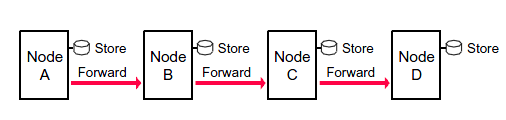
\includegraphics[scale=0.6]{2-background/img/store-and-forward.png}
    \caption{\textit{Store-and-forwarding} technique example}    
    \label{fig:store-carry-forward}
  \end{center}
\end{figure}

Messages are stored in storage mediums which can hold them for a long time period called persistent storage. This is another difference with internet protocols, where routers adopt very short-term storage provided by memory chips to store incoming packets. In Internet routers messages are queued only for a few milliseconds while they are waiting for their next hop. In DTNs routers need persistent storage for one or more of the following reasons:
\begin{itemize}
\item A communication link to the next hop may not be available for a long time and during this period message must be stored in the router.
\item There could be asymmetries in speed and reliability between nodes, so one node in a communicating pair may send or receive data much faster or more reliably than the other node.
\item A message, once transmitted, may need to be retransmitted if an error occurs at an upstream node or link, or if an upstream node declines acceptance of a forwarded message.
\end{itemize}


 
\section{Peer-to-Peer networks}
The most distinctive difference between Client/Server networking and Peer-to-Peer (P2P) networking is the role of each node in the network. In Peer-to-Peer networks nodes act as Servent, which is is an artificial word derived from the terms server and client. This term represent the capability of the nodes of a Peer-to-Peer network of acting at the same time as server as well as a client. In Client/Server networks each node can act as a server or as a client but cannot embrace both capabilities.
\\

In \cite{Aberer02anoverview} are identified three principles underlying P2P networks:
\begin{itemize}
\item  \textbf{Principle of sharing resources}: P2P systems involve an aspect of resource sharing, such as disk space network bandwidth or services. By sharing of resources applications can be realized which could not be set up by a single node. This was the driving motivation
behind a P2P system such as Napster.
\item \textbf{Principle of decentralization}: this is an immediate consequence of sharing
of resources. Parts of the system or even the whole system are no longer op-
erated centrally. Decentralization is in particular interesting in order to avoid
single-point-of failures or performance bottlenecks in the system. Examples
of fully decentralized systems are Gnutella and Freenet.
\item \textbf{Principle of self-organization}: when a P2P system becomes fully decen-
tralized then there exists no longer a node that can centrally coordinate it’s
activities or a database to store global information about the system centrally.
Therefore nodes have to self-organize themselves, based on whatever local in-
formation is available and interacting with locally reachable nodes (neighbors).
The global behaviour then emerges as the result of all the local behaviours
that occur.

\end{itemize}




\subsection{Peer-to-Peer networks as Overlay networks}
Peer-to-peer networks are typically constructed as overlay networks. These are computer networks which are built on top of other networks, adding an additional level of routing-logic. This is often done in the application layer, above transport and network layers, where maintenance and management algorithms operate. Overlays usually define some set of functions to forward overlay packets using this state. In order to implement such a higher-level of routing, many overlay networks define an additional level of logical routes above routes provided by the network layer. Each logical route can be composed by multiple lower-levels routes, i.e. routes composed by several IP-level routes.
\\

Overlay networks provide design flexibility and ease of deployment, at the cost of little inefficiency compared to a system implemented directly in coordination with the network layer. Also, designing a system using overlays helps to focus on the problem and functionalities to provide. While overlays are positioned at the application layer, it is possible to think to them as a distinct layer implementing higher-lever routing and transport services, while the complexities of network-level routing and transport are encapsulated in the lower layers.
\\

This allows to implement new services that are not yet available within the existing network. Some examples are the Distributed Hash Table (DHT) or the implementation of Virtual Private Networks (VPNs). 


%It also separates design concerns. Indeed, while overlays are positioned at the application layer, it is more fitting to think of them as a distinct layer implementing higher-lever routing and transport services. This separation of concerns partially decouples design, implementation, and optimization from the network and transport layer. The programmer is then free to focus solely on whatever problems are at hand, while the complexities of network-level routing and transport are encapsulated in the lower layers.
%\\

%The use of an overlay network in the design of new Internet services bypasses the need for strong social coordination during deployment. This has proven important in the continued evolution of the network, as individual autonomous systems and end-users can begin (or end) providing services in a piece-wise fashion. Multicast serves as a strong example of why such piece-wise role out is critical for eventual deployment.

\subsection{Peer-to-Peer architectures}
One ways to classify P2P networks is to consider the degree of centralization of the network and divides P2P networks in centralized or decentralized (or unstructured) networks.
\\

\paragraph{Centralized P2P networks} One of the most famous occurrence of the P2P paradigm was probably Napster\cite{Carlsson:2001:RFN:647728.734520}. This file-sharing system used an architecture in which a centralized entity provides a directory service to all participating peers, effectively forming a star network. All peers joining the system have to register their data with this centralized server. This allows other peers in the system to locate any data in the network by presence of a physically centralized directory. Only pointers to decentralized available peers are stored at the centralized server while the actual data is store in peers. When a peer found a pointer to relevant data in the directory, it could directly communicate with other peers that store the data in a decentralized manner, completely bypassing the centralized directory entity. Napster cannot be denoted as a pure P2P system because without central directory servers, single peers are not able to find resources shared by other peers.
\\

\paragraph{Decentralized P2P networks}
In decentralized (or unstructured) P2P architectures peers do not rely on any centralized entity to locate data items within the network. More specifically, in decentralized P2P networks, peers recursively forward received requests to neighbouring peers, in an attempt to find all relevant items in the network. This request forwarding is done using a broadcast technique know as message flooding. To prevent infinite loops and to control the number of messages generated by one single request, each message gets assigned a time-to-live (TTL) value. Each peer forwarding such a message decreases this value by one, and only messages with positive TTL values get forwarded. The main advantage of unstructured P2P networks is the fact that there is no need to maintain a network structure, as peers maintain only pointers to a limited number of direct neighbours. Also there is no need for a specific storage location for data items, as they can be located anywhere in the network.
\\

In \cite{Schollmeier:2001:DPN:882470.883282}, R. Schollmeier splits P2P networking
definition into two sub-definitions: \textit{pure} and \textit{hybrid} Peer-to-Peer networks.\\ 
The network is said pure if any peer in the underlying topology can be added and removed arbitrarily without having the network suffering any loss of network service. In other words, there is no special set of nodes that must be present for the service to work. \\
Peer-to-peer networks and algorithms in which an essential subset of peers exists are said to be hybrid networks. Hybrid networks typically have one or more strongly differentiated roles for various subsets of peers. Often role differentiation is related to the class of resource being shared. For example, one set of peers may handle storage, and another provide computational power. \\
%In other networks roles are differentiated across functionality, as is done in peer-to-peer file-sharing services such as Napster and BitTorrent, both of which separate indexing, and storage and download.
Pure peer-to-peer networks tend to generalize better, since they do not require any centralized, essential node to provide the related service.

%\section{Related works}
% ---------------------------------------------------------------------------
%: ----------------------- end of thesis sub-document ------------------------
% ---------------------------------------------------------------------------


% this file is called up by thesis.tex
% content in this file will be fed into the main document

%: ----------------------- name of chapter  -------------------------
\chapter{M2MShare}\label{m2mshare} % top level followed by section, subsection


%: ----------------------- paths to graphics ------------------------

% change according to folder and file names
%\graphicspath{{2-Consorzi/images/}}


%: ----------------------- contents from here ------------------------
In DTNs mobility and low node density require new strategies to implement a file-sharing application which allow the exchange of multimedia contents between mobile devices. M2MShare \cite{tesiarmir} uses Bluetooth to create a Peer-to-Peer overlay network and uses node mobility to reach data content on other local disconnected networks. The main idea of this protocol is to use a store-delegate-and-forward model. This is similar to the store-and-forward strategy widely used in DTNs, but M2MShare adds the \textit{delegate} part to the model. The result is an asynchronous communication model where a peer delegates an unaccomplished task to other peers in the overlay network.
\\

Delegations are used to extend search and diffusion area for a shared file, while M2MSHare dynamically establishes forward routes along the destination path by exploiting social relations existing between peers users. This is done by limiting delegations only to frequently encountered peers, which users can pass on by the same geographical location at the same time frequently enough. The history of previous encounters is then used as heuristic evaluation of whether a peer is a good candidate for delegations. This allows assigning tasks only to nodes that we should meet again in the future, so they can return the result of the task back to us.
\\

In this chapter we describe the protocol from a top-down prospective, showing some details about the modules (\figurename~\ref{fig:stack-M2MShare}) which compose M2MShare architecture. 

\begin{figure}[htpb]
  \begin{center}
    \includegraphics[scale=0.6]{3-m2mshare/img/stack.png}
    \caption[M2MShare protocol stack \cite{articoloM2MShare}]{M2MShare protocol stack. Blocks shown in gray are proprietary.\cite{articoloM2MShare}}    
    \label{fig:stack-M2MShare}
  \end{center}
\end{figure}
%
%Mobility and low node density require a revision of networking protocols toward a delay tolerant approach. In this section we expose some operational details of M2MShare, the application we designed and implemented to demonstrate the opportunistic DTN approach in mobile to mobile multimedia content sharing.
%
%M2Mshare uses the Bluetooth to create a P2P overlay networks, which would allow the automatic exchange of multimedia content among smartphones. Our software automatically initiates a search by broadcasting the user’s query request toward other Bluetooth enabled devices operating the program. Once the answer/s is received, data found to match the criteria will be automatically requested for download. All this process is done without the user mediation; the user only needs to specify the search terms, configurable through the user interface and chose from the matched content list. Key features of M2MShare are its ease of use and autonomy, once the initial preferences are set up no further user interaction is needed and the user can find downloaded files directly on her/his phone, when done.
%Given that energy consumption is a problem for handheld devices the notion of active sessions was introduced. An active session is a period of time in which the software is functional and performs its duties and such periods are configurable through the graphical user interface. This way, the user can set the application to look for requested contents only in certain periods of the day; for instance, when commuting or during lunch time in the cafeteria, so as to be active only when it could be useful since the high number of other peers around.
%
%M2MSHare uses node mobility to reach data content on other local disconnected networks. This is achieved by introducing an asynchronous communication model, store-delegate-and-forward where a peer delegates and unaccomplished/unsatisfied task to other peers in the overlay network. M2MSHare dynamically establishes forward routes (delegations) along the destination path by exploiting social relations existing between users operating mobile wireless devices, whose activity is entirely user-transparent Delegating tasks to all encountered peers is energy and bandwidth consuming. Also, it would be useless to assign tasks to peers that will never be met again in the future. To avoid this M2MShare exploits social relations and delegates tasks only to frequently encountered peers, peers whom are expected to be encountered again in the future.
%
%We could say that we exploit social relations among users to determine possible task delegates. This is not a new approach as context and social relations are already studied in opportunistic data transmission. Yet, we utilize even unknown social relations by connecting users that have to pass by the same geographical location at the same time frequently enough. To assume that a candidate for task delegation could be met again in the future (so that she/he will be able to deliver contents possibly found), we use as an heuristic the history of previous encounters.

\section{DTN module}
DTNs are particularly useful in situations with intermittent connectivity and long and unpredictable intervals in contacts between nodes. Routing protocols developed for and used in the Internet are not suitable for use in mobile networks, where every node has a limited connection range and high mobility. These factors make it difficult, and sometimes impossible, to establish an end-to-end connection between source and destination nodes.
\\

In a Peer to Peer application it is also fundamental to have a high availability of shared files, to ensure the recovery of a searched file. This implies the need for a high number of simultaneously connected nodes, which we saw was not so obvious in a mobile network.
\\

To overcome these limitations, M2MShare uses an asynchronous communication strategy in which a \textit{client} peer, in search for a file, can delegate to another peer, a \textit{servant}, the task of searching for the file and returning it to the requester. Delegation system is at the root of M2MShare. This permits widely extending the area of where to look for the searched file, in a network composed of spread out and poorly connected nodes.
\\

Before proceeding further it would be useful to explain in what a delegation action consists of. A delegation is the action performed by a client peer which asks a servant peer to execute some unaccomplished task of its own. This unaccomplished task can be a query, composed of several keywords, for which the client wants to receive a list of files which satisfy it. To accomplish this task, the servant schedules it for later execution and searches among shared files in encountered nodes for some file satisfying the query. When the pending task is completed, the servant creates a new task type, a forward task. The objective of this kind of task is to return the output of a pending task to the requester node. 
\\
One task can be delegated by the client to several servant peers and this allows using nodes mobility as an advantage instead of a negative factor. A client node can virtually enter in contact range with nodes that it would never otherwise meet.

All delegated tasks also have a Time To Live (TTL) value. If a delegated task is not completed and its result has not been returned to the client within its TTL value the task expires, it is deleted and not scheduled again for execution in the servant.
\\

\subsection{Servant Election}
The entire task life-cycle is done in an infrastructure-less environment, where routing paths are dynamically created during execution. Therefore it is important to choose wisely which peers can be elected as servants.
\\

The simpler choice would be to delegate an unaccomplished task to every met node. This might not be a good strategy in servant election. Delegating a task to every met node would be very expensive in bandwidth usage and in energy consumption. These factors are very important in a mobile environment where nodes have limited energy autonomy. 
\\

A possible solution would be to analyse common interests between client and other peers. \cite{socialNetworks} shows a strategy for data diffusion in which a node shares only certain kinds of data to another node, accordingly to their common interests and relationship. If the other peer is a friend it would be convenient to share data related to their common interests. If the other is not a friend node, the client node would share the data most different from their common interests.
\\

Once the task has been delegated it is then fundamental that its result is forwarded back to the client. Otherwise the delegation would be useless. M2MShare strategy is to elect as servants only nodes that we expect to meet again. As we will see in Section \ref{descrWDM}, related to Working Day Movement model, one person's daily activities can highlight a repetitiveness in movements and met people. Spontaneous and temporary \textit{communities} are created by people who meet regularly, i.e. colleagues who work in the same office, commuters who use the same transportation to reach their work place, etc..
\\

The idea behind M2MShare is that a frequently encountered person is a person that we will probably meet again and therefore it is a good candidate for servant election. To evaluate how frequently a node will meet another node, M2MShare uses an active daemon called \textit{PresenceCollector}, described in Section \ref{descrPresenceCollector}. This daemon traces the number of encounters, scanning at regular intervals for other nodes within communication range. When the number of encounters with another node exceeds the value of a parameter called \textit{Frequency Threshold}, that node is elected as servant.
\\

The numbers of encounters with other peers are saved in a list with limited length. This limitation is adopted to guarantee limited memory usage. To allow each peer the possibility to serve as servant, a replacement strategy is adopted for entries in encounter list. When a peer is elected as servant, its entry is removed from the list. If a peer is not elected as a servant and its entry remains on the list for a long time period, then it is removed from the list. The maximum time a peer can be on the list without being elected as servant is related to a value called \textit{Probation Window}. If the list is full and a new peer is encountered, its information is discarded. A new peer can enter in the list only when a slot is freed by the replacement strategy.

\section{Search module}
Before a user can choose what file to download from the network, it must know what files are shared by other users and find what it is looking for in them. Every peer in the network maintains a local repository of files shared with other M2MShare users. For every file information is available about file name, dimension, position in local file system and an hash value that univocally identifies that file in the network.
\\

There are two kinds of file queries: 

\begin{description}
\item[Unique file query:] a single file is searched and a boolean answer (present / not present) is needed.
\item[Keyword query:] the user asks for a list of files satisfying some keyword included in the query.
\end{description}

To satisfy a keyword query, M2MShare uses the Inverted Index List strategy. Every shared file is indexed under a finite number of terms contained in the file description text and during a query execution the Search module looks in these terms for files suitable for the response.


\section{Transport module}
M2MShare operates on devices with limited memory and calculation resources. Each device must simultaneously handle incoming requests for uploads and delegations from other peers and user requests issued on the device itself. If these requests were executed in parallel, then each one would require a separate execution flow. With the limited device resources, this could cause substantial memory usage and consequently, probably crash the application.
\\

In Transport Module, M2MShare manages active tasks queuing, and executing only a limited number of them simultaneously. Tasks are divided in different kinds and this permits applying different policies to different types of requests. These policies are implemented using different task queues and a component called \textit{QueuingCentral} which manages the queues. It also imposes limits on the maximum number of tasks a single peer can handle.
\\

When a task is created or received from another peer delegation, it is queued in the related queue and scheduled for later execution. The queues managed by the QueuingCentral are:
\begin{description}
\item[dtnDownloadQueue:] includes remote tasks which indicate that a servant peer has completed a previously delegated task.
\item[dtnPendingQueue:] includes tasks previously delegated from other peers. The current peer acts as servant for these tasks.
\item[dtnPendingUpload:] includes completed tasks previously delegated from other peers. The current peer is ready to forward the result of these tasks.
\item[queryQueue:] includes user-issued queries.
\item[uploadQueue:] includes data requests from other peers.
\item[virtualFileQueue:] includes user-issued file download requests.
\end{description}

Tasks execution is scheduled by a component called \textit{Scheduler}, which extracts tasks from related queues and executes them. Inside each queue tasks are inserted and fetched with a FIFO policy. The Scheduler includes four execution flows used to implement inter-queue policies and to assign different priorities to different task types. Some tasks can use several execution flows, with a maximum number of flows for each task. This permits, for example, simultaneous downloading of pieces of the same file from different sources.
\\

One of the highlights of M2MShare is task delegation. This is done by remotely communicating task informations to a servant peer. The task, when active, is encoded using serialization on the client side, transmitted to the servant peer and there the task is decoded and queued to the correct queue related to pending tasks.

%Provides the task queuing mechanism and task lifecycle management. We discuss about the necessity of resource management given the fact that mobile devices are resource constraint and extend our solution to this. An important part of this section is the communication protocol that individual tasks implement along with a detailed analysis of the data packets exchanged during communication. Finally, we introduce the file division strategy and provide some test results that demonstrate its efficiency over other division strategies


\section{Routing module}
M2MShare uses this module for query routing, using a relay method borrowed from ORION \cite{orion}. In every node, a structure similar to ORION File Routing Table is used to store alternative paths to file shared in remote peers. The usage of this structure allows to keep file locations transparent to the requester node. From its point of view, all files are shared by in-reach area nodes, while these act as relay nodes during file transfers.\\
A flood control mechanism is implemented using a technique borrowed from AODV \cite{aodv}. Query requests are uniquely identified and every node maintains an \textit{ID} which is incremented on each broadcast issued. When a node receives new requests, it checks to see if the request has been already forwarded, before broadcasting it.



\section{MAC module}
\label{descrPresenceCollector}
We saw that a node must be met several times before being elected as a servant. To evaluate if a peer is a frequently encountered peer and eventually elect it as a servant, M2MShare uses a daemon called \textit{PresenceCollector}, which periodically scans the network for in-reach area devices. 
\\

Scan frequency is a very important parameter. It influences energy consumption and probability for another peer to be elected as a servant. The presence collector is always active, so a high scan frequency is not reasonable because it results in waste in the network bandwidth and device energy. Also, a high frequency results in a high probability that a node will be elected as a servant: the number of encounters raises and the \textit{Frequency Threshold} is exceeded faster than with a low scan frequency value.
\\

While scan frequency can be set by the user, additional efforts have been made to automatically tune the \textit{Frequency Threshold} value. This is the other parameter that affects the probability of a node being elected as a servant: a few encounters are enough, with a low value, to exceed the threshold value. If the value is too low, we might delegate a task to peers that we would never meet again, resulting in the results of the task never being forwarded. On the other hand, with a high \textit{Frequency Threshold} value, many promising peers might be rejected from being elected as servants.
\\

At the beginning of every day, M2MShare uses a tuning algorithm which adapts the \textit{Frequency Threshold} value according to the observations made during the previous day. Considered values are the number of elected peers and \textit{Probation Window} value. A peer is considered frequently encountered if it is met a number of times greater than the \textit{Frequency Threshold} in a period as long as the \textit{Probation Window} value. After this period, if a peer has not yet been elected, it is removed from the encounter list. If \textit{Probation Window} value is high and few nodes are elected, the  \textit{Frequency Threshold} is lowered, making it more probable for a node to be elected. On the other hand, if the number of elected peers is too high, the \textit{Probation Window} is lowered. When its value reaches the minimum value (set to 2 days), the \textit{Frequency Threshold} is raised.


\section{File Division Strategy}
\label{descrFileDivisionStrategy}
Bluetooth file transfer applications usually adopt a client-server paradigm where devices pair with each other for the entire duration of data transfer. If the transfer is interrupted, exchanged data is of no use. This is because every file transfer has to start from the beginning. 
\\

In a mobile environment such as the one where M2MShare operates, disconnections between nodes are very frequent. The standard file transfer strategy is not suitable for this environment, because pairing for the entire duration of data exchange could be very difficult. We must remember that M2MShare should be entirely user transparent, so the user need not worry about file transfers. Data exchange should run automatically whenever possible and the transfer strategy should adopt transfer resume.
\\

M2MShare provide a file division strategy where files are divided in intervals of variable size. The file is seen as a map of non overlapping intervals of variable length that need to be downloaded. So, when one node asks another node for a file, it asks only for not yet downloaded intervals. If a disconnection occurs, the download can restart with the remaining not yet downloaded intervals.
\\

One of the characteristics of this file division strategy is the starting point of file transfers. If every file transfer starts from the beginning of the file, with several file possessors in the area of reach, there would be overlapping downloaded intervals downloaded. Overlapping data is of no use, creating redundancy, and M2MShare file division strategy tries to minimize that redundancy. This is done by assigning a different \textit{download map} to each file possessor. A download map is a list of not yet downloaded intervals, with a starting point which identifies the interval from which to initiate fetching data. The starting point is calculated by considering the number of intervals the file is composed of, the length of the file and the index of the next interval to be fetched. For additional details refer to \cite{tesiarmir}.
\\

The fact that each file possessor is asked for the file starting from different points allows reconstructing the whole file even if just part of it is downloaded from each of them. When the requested interval has been downloaded, if the file possessor is still in reach, the rest of the map is requested. In case of task delegation, a data download might be delegated to a servant peer, and in this case the entire download map is communicated to the servant device.
 
 
% ---------------------------------------------------------------------------
%: ----------------------- end of thesis sub-document ------------------------
% ---------------------------------------------------------------------------


% this file is called up by thesis.tex
% content in this file will be fed into the main document

%: ----------------------- name of chapter  -------------------------
\chapter{Modelli di movimento}\label{movimento} % top level followed by section, subsection


%: ----------------------- paths to graphics ------------------------

% change according to folder and file names
%\graphicspath{{2-Consorzi/images/}}


%: ----------------------- contents from here ------------------------
Uno degli aspetti pi� importante per garantire la realisticit� di una simulazione riguarda il comportamento dei nodi, in particolare il loro movimento. Come � facile intuire, in una DTN i cambiamenti di posizione dei vari nodi influiscono pesantemente la connettivit� e quindi le prestazioni dell'intera rete. Proprio per questo motivo � fondamentale simulare il pi� realisticamente possibile il comportamento dei nodi all'interno della simulazione.
\\

Il simulatore TheONE contiene al suo interno diversi modelli di movimento che possono essere assegnati ai vari gruppi di nodi. Presenter� ora un breve riassunto dei modelli a disposizione, soffermandomi in particolare su quello scelto per le simulazioni svolte, ossia il Working Day Movement Model (WDM)

\section{Random Map-Based Movement}
Il modello pi� semplice fra quelli disponibili � il Random Map-Based Movement (RMBM). I nodi che adottano questo modello si muovono in maniera casuale ma sempre seguendo le strade descritte dalla mappa della simulazione. Il risultato di questa modalit� � un movimento troppo casuale per simulare accuratamente il comportamento unmano per quanto riguarda la mobilit�.

\section{Shortest Path Map-Based Movement}
Lo Shortest Path Map-Based Movement (SPMBM) � un modello leggermente pi� realistico rispetto a RMBM. In questo modello i nodi scelgono casualmente un punto di destinazione all'interno della mappa e seguono la via pi� breve per raggiungerlo dalla posizione attuale, sempre seguendo le strade descritte dalla mappa della simulazione. Le destinazioni possono essere scelte in maniera completamente casuale o da un insieme di Punti di Interesse, in modo da simulare l'attrazione delle persone per luoghi come punti di ristoro, negozi o attrazioni turistiche.

\section{Routed Map-Based Movement}
Un modello che invece della casualit� nel movimento utilizza dei persorsi predeterminati � il Routed Map-Based Movement (RMBM). I nodi che adottano questo modello si muovono lungo rotte predefinite, per tutta la durata della simulazione, rendendo RMBM utile per rappresentare degli spostamenti ripetitivi, come ad esempio quelli di autobus, tram o treni.

\section{Working Day Movement Model}
Il modello pi� realistico � senza dubbio il Working Day Movement Model (WDM). Come il nome pu� fare intuire, questo modello simula i movimenti di 
\\

\subsection{Home Activity Submodel}

\subsection{Office Activity Submodel}

\subsection{Evening Activity Submodel}

\subsection{Transport Activity Submodel}

I Consorzi di bonifica sono, infatti, enti che si autogovernano (in quanto sono i consorziati, cio� quelli che pagano, ad eleggere i proprio amministratori ed a decidere cosa fare) e che si autofinanziano, cio� non dipendono dalla Regione o dallo Stato per i soldi necessari a garantire la manutenzione e l'efficienza delle opere. Nei Consorzi sono da sempre attuati quelli che oggi si direbbero "decentramento amministrativo" e "federalismo fiscale".
\\
Tra le attivit� quotidiane del Consorzio ritroviamo il funzionamento degli impianti di sollevamento, la pulizia dei corsi d'acqua in gestione, l'espurgo dei canali, la difesa idraulica, la manutenzione delle siepi, il restauro di antichi manufatti idraulici.
\\
Il personale di campagna e l'ufficio tecnico curano giornalmente il buon funzionamento di tutti gli impianti di sollevamento e delle altre opere idrauliche compresa la rete di scolo e quella di distribuzione irrigua.
\\
Lo sfalcio e la pulizia dei corsi d'acqua consorziali sono effettuati nel corso di tutto l'anno su una rete di corsi d'acqua di 26.050 chilometri.
\\
Un continuo espurgo e la pulizia degli alvei dei canali sono finalizzati a garantire la necessaria funzionalit� della rete salvaguardando il territorio dai possibili fenomeni di sommersione e allagamento.
\\

La difesa di sponde, salti di fondo, ponti ed altre opere sono realizzati per limitare le erosioni per contribuire alla sicurezza idraulica dei territori attraversati dai corsi d'acqua. Molti lavori vengono eseguiti con la collaborazione delle Amministrazioni comunali appartenenti al comprensorio del Consorzio.
\\
La riqualificazione paesaggistica attraverso l'incremento dell'arredo arboreo di campagna, la messa a dimora di specie arboree ed arbustive, la ricostituzione delle siepi ripariali, determinano un beneficio di ordine sia naturalistico che ambientale.

\figuremacro{consorzi}{Mappa dei Consorzi del Veneto}{}{}

\section{Il Consorzio Bacchiglione Brenta}
Il Consorzio di bonifica Bacchiglione Brenta ha sede in Padova.
Il comprensorio del Consorzio di bonifica Bacchiglione Brenta ricade nelle provincie di Padova e Venezia, interessando una superficie complessiva di 58.247 ettari, il 20,27\% della quale risulta urbanizzata.
I Comuni interessati al territorio consortile sono 39, di cui 31 nella provincia di Padova. 
Il comprensorio � suddiviso in 10 bacini idraulici.
\\

Le aree a deflusso naturale sono 23.999 ettari (41,2\%), quelle a deflusso meccanico di 14.350 ettari (24,64\%), quelle a deflusso alternato (scolo naturale e scolo meccanico) di 19.898 ettari (34,16\%).
Le superfici idraulicamente sofferenti sono all'incirca pari a 10.250 ettari (17,60\%), mentre le superfici ad allagamento certo senza azioni di pompaggio da parte del Consorzio sono all'incirca di 20.000 ettari (34,34\%).
Il Consorzio Bacchiglione Brenta gestisce 37 impianti di sollevamento (idrovore) con una quantit� di acqua sollevata pari a 70 milioni di mc/anno e un consumo assorbito pari a 1,034 milioni di kWh (quinquennio 2003-2007).
L'estensione della rete idraulica consortile � di 884 chilometri, dei quali 291 (32,92\%) risultano ad esclusivo uso scolo, 30 (3,39\%) ad uso esclusivamente irriguo e i rimanenti 563 (63,69\%) ad uso misto scolo e irrigazione.
La superficie irrigata interessa 15.732 ettari (il 27,01\% della superficie consortile); l'intera superficie irrigata presenta un'irrigazione con metodo di soccorso (irrigazione attuata per impedire a condizioni climatiche avverse di rovinare il raccolto).
\\

I consorziati sono 169.474 per un introito complessivo di 7.903.913 euro, di cui 5.587.939 euro sono relativi alla contribuenza extragricola (70,70\%) e 2.315.974 euro relativi alla contribuenza agricola (29,30\%).
Le unit� lavorative presenti nel Consorzio sono 81.
\\

I dati dei sensori ambientali del Consorzio Bacchiglione Brenta sono stati utilizzati per avviare la sperimentazione del progetto.

\section{Sensori ambientali}
I Consorzi gestiscono una serie di impianti volti alla sicurezza idraulica e alla distribuzione irrigua. Per la gestione di tali impianti � indispensabile monitorare costantemente la situazione idrica e meteorica del territorio al fine di prevenire o limitare fenomeni dannosi quali piene o, all'estremo opposto, fenomeni di siccit�. A tale scopo nel territorio consortile, ed in particolare in prossimit� degli impianti, sono installati appositi sensori adibiti al monitoraggio del livello dei fiumi, della temperatura, dell'umidit�, delle precipitazioni meteoriche. Vediamo pi� in dettaglio due di questi, utilizzati nella sperimentazione del progetto: l'idrometro e il pluviometro.
\\

L'idrometro � lo strumento necessario per poter rilevare le quote idrometriche, cio� l'innalzamento o l'abbassamento del livello dell'acqua dei fiumi o dei laghi.
Il pi� semplice degli idrometri � quello ad asta che � costituito appunto da una barra, generalmente in lega metallica per poter resistere alla corrosione, contrassegnata da tacche numerate che riportano i progressivi riferimenti all'unit� di misura in vigore (metro, centimetro, ecc.) e posta verticalmente a diretto contatto con l'acqua del fiume, spesso fissata ad una spalla o ad una pila di un ponte o di una banchina fluviale.
Attualmente vengono utilizzati strumenti pi� complessi e sofisticati (idrometrografi, teleidrometri) che utilizzano tecnologie pi� moderne (laser, ultrasuoni, ecc.) per effettuare le letture idrometriche e per raccogliere e trasmettere i relativi dati a distanza ed in tempo reale.
\\

Per "livello idrometrico" in un determinato luogo del fiume si intende la misura del dislivello tra la superficie dell'acqua di un fiume ed un punto di riferimento altimetrico che pu� essere il livello medio del mare (l.m.m) oppure il riferimento "zero" dell'idrometro stesso (detto "zero idrometrico").
Lo zero dell'idrometro altro non � che la quota altimetrica (sempre sul livello medio del mare) che si � convenuta per quell'idrometro stesso.
\\

L'idrometro � un valido aiuto per l'attivit� di salvaguardia del territorio contro i pericoli conseguenti alle piene dei fiumi, poich� � il monitoraggio dei livelli idrometrici che consente di fare previsioni sull'andamento degli eventi di piena e prendere le misure del caso, quali attivare un impianto di scolo o, in casi estremi, allertare gli organi di protezione civile.

\figuremacro{idro}{Idrometro}{Un esempio di idrometro nella sua forma pi� semplice. Per monitorare i livelli dei fiumi i Consorzi utilizzano ad oggi pi� sofisticati idrometri elettronici in grado di comunicare la lettura a distanza.}{}

Il pluviometro � lo strumento utilizzato per misurare la quantit� di pioggia caduta. Fino a circa 10-20 anni fa si indicavano come pluviometri quegli strumenti che di fatto non avevano modo di registrare l'evoluzione temporale della pioggia e che venivano controllati a cadenza quotidiana. Diversamente il pluviografo era uno strumento che riusciva, mediante un sistema di registrazione meccanico, a riportare graficamente la quantit� di pioggia caduta in un certo intervallo di tempo (giornaliero, settimanale, ecc), su un'apposita striscia di carta millimetrata. Con questi strumenti era possibile arrivare a risoluzioni temporali massime dell'ordine di cinque minuti, anche se nella maggioranza dei casi la risoluzione utilizzata era nell'ordine della mezz'ora. Ovviamente la registrazione di un evento di pioggia con questo sistema comportava una serie di problemi di manutenzione, affidabilit� degli strumenti, lettura e trattazione dei dati che doveva essere fatta comunque a mano. Con lo sviluppo dell'elettronica prima e dell'informatica poi, i pluviografi sono andati sempre pi� affermandosi dato che acquistavano facilit� di gestione e di utilizzo, soprattutto perch� si passava da strumenti meccanici a strumenti elettronici con la possibilit� di archiviare i dati in maniera digitale. I pluviometri utilizzati attualmente sono costituiti da un imbuto che porta acqua in una doppia vaschetta metallica o di plastica, incernierata in un punto. � un sistema il cui equilibrio varia a seconda di quanta acqua c'� nelle vaschette. Il ribaltamento avviene per 0,2 mm, quindi ogni volta che cadono 0,2 mm di pioggia si ribalta. Tale vaschetta � collegata ad un sistema elettronico che registra i ribaltamenti; i dati possono venire in seguito spediti ad un server centrale che immagazzina tutti i dati raccolti. Con questo strumento si pu� effettuare la misurazione anche in caso di neve: l'imbuto viene munito di resistenza termica, che scioglie l'acqua (in fase solida), riduce il volume misurato ad 1/10 della neve e misura l'equivalente in acqua.

\figuremacro{basculla}{Pluviometro elettronico}{}{}

 
% ---------------------------------------------------------------------------
%: ----------------------- end of thesis sub-document ------------------------
% ---------------------------------------------------------------------------


% this file is called up by thesis.tex
% content in this file will be fed into the main document

%: ----------------------- name of chapter  -------------------------
\chapter{ONE - L'ambiente di simulazione}\label{simulatore} % top level followed by section, subsection


%: ----------------------- paths to graphics ------------------------

% change according to folder and file names
\graphicspath{{2-simulatore/img/}}


%: ----------------------- contents from here ------------------------
L'ambiente scelto per svolgere le simulazioni è The ONE (Opportunistic Network Environment) versione 1.4.1, descritto in \cite{articoloONE}. Questo simulatore scritto in Java è completamente configurabile e permette di simulare il movimento dei vari nodi partecipanti alla simulazione, gestire le connessioni e lo scambio di messaggi fra i vari nodi (utilizzando diversi protocolli di routing) e visualizzare sia i movimenti che il traffico dati nell'interfaccia grafica di cui dispone.
\\

Per quanto riguarda il movimento, il simulatore può accettare in input tracce provenienti da registrazioni dal mondo reale, dati creati tramite generatori di movimento esterni oppure crearli dinamicamente tramite dei modelli di movimento, alcuni dei quali descritti più nel dettaglio in [movimento]. Sia i modelli di movimento che i vari protocolli di routing vengono gestiti come moduli indipendenti e vengono caricati a seconda di quanto impostato in fase di configurazione. Ciò permette una semplice implementazione di nuovi protocolli di routing e modelli di movimento all'interno del simulatore.
\\

Il simulatore permette infine di salvare dati statistici riguardanti le simulazioni svolte tramite la generazione di report, anch'essi gestiti in maniera totalmente modulare e configurabile.
\\

\section{Configurazione}
\label{configurazioneONE}
Una determinata simulazione viene impostata creando dei files di configurazione che descrivano i vari aspetti dello scenario, dalla durata della simulazione al numero di nodi che la compongono, fino alle caratteristiche specifiche di ogni gruppo di nodi. Tali files di configurazione sono dei semplici files di testo in cui vengono impostati i parametri relativi allo scenario, ai modelli di movimento e ai protocolli di routing. I valori impostati verranno caricati dinamicamente ed andranno ad attivare e configurare i moduli che si è scelto di utilizzare per la simulazione corrente.
\\

All'interno dei files di configurazione, i parametri sono salvati come coppie chiave-valore. La sintassi della maggior parte delle variabili è del tipo

\begin{center}
\textit{Namespace.chiave = valore}
\end{center}

Il namespace indica generalmente a quale parte dell'ambiente di simulazione la variabile si riferisce. Più nello specifico il namespace indica (nella quasi totalità dei casi) la classe Java che andrà a leggere quel parametro. durante la fase di inizializzazione. Questa convenzione è utilizzata soprattutto dai moduli relativi ai modelli di movimento e ai protocolli di routing, quindi è bene che venga utilizzata nella realizzazione di nuovi moduli da aggiungere al simulatore.
\\

Per facilitare la lettura e la configurazione, i valori numerici possono utilizzare i suffissi kilo (k), mega (M) o giga (G), assieme al punto \textquotedblleft .\textquotedblright come separatore decimale. I parametri di tipo booleano invece accettano i valori \textquotedblleft true\textquotedblright
 o \textquotedblleft 1\textquotedblright , \textquotedblleft false\textquotedblright o \textquotedblleft 0 \textquotedblright .
 \\
Dei commenti possono essere inseriti nei files di configurazione utilizzando il carattere \textquotedblleft
\#\textquotedblright, che ottiene il risultato di far saltare il resto della riga durante la fase di lettura.
\\

Per ogni simulazione ci possono essere più files di configurazione, in modo da poter dividere i parametri in più categorie, ad esempio in un file inserire i parametri relativi allo scenario, con le strade e i quartieri in cui è diviso, in un altro file configurare i nodi con le caratteristiche tipiche di ogni gruppo, in un altro ancora selezionare i report da generare durante l'esecuzione e così via. Il primo file di configurazione letto, se esiste, è sempre il file \textquotedblleft default\_settings.txt\textquotedblright e negli altri files di configurazione è possibile definire nuovi parametri o sovrascrivere alcuni di quelli definiti nei files precedenti. Ciò permette di definire in alcuni files dei parametri generali, validi per tutte le simulazioni, e variarne altri cambiando solo gli ultimi files di configurazione.
\\

All'interno dello stesso scenario, i nodi sono divisi in più gruppi, composti da un numero variabile di nodi. All'interno di un gruppo, tutti i nodi condividono delle caratteristiche comuni, dal protocollo di routing utilizzato, al modello di movimento, ai tipi di interfacce disponibili per la comunicazione. E' possibile impostare inoltre delle caratteristiche comuni a tutti i gruppi in modo da non dover ripetere la definizione di alcuni parametri per tutti i gruppi. La variazione di caratteristiche fra un gruppo e l'altro permette di ottenere dell'eterogeneità fra i comportamenti simulati all'interno dello scenario.
\\

Nei files di configurazione utilizzati da ONE è possibile inoltre impostare array di valori per ogni parametro: ciò permette, durante una serie di esecuzioni batch, di ottenere automaticamente una serie di simulazioni che differiscono l'una dall'altra per alcune impostazioni di parametri, automatizzando notevolmente la raccolta di dati con configurazioni differenti dello stesso scenario.
\\ In questo caso la sintassi sarà del tipo

\begin{center}
\textit{Namespace.chiave = [valoreEsecuzione1; valoreEsecuzione2; valoreEsecuzione3; ecc]}
\end{center}

Alcuni parametri, infine, accettano come valore il percorso di un file e in questo caso può essere espresso sia in maniera assoluta che relativa. Un esempio di variabili che necessitano di questo tipo di valori sono le mappe, per cui si impostano i files che le contengono, o gli input per i generatori di eventi, per i quali i files da caricare descrivono gli eventi da creare durante la simulazione.

\section{Visualizzazione}
La principale modalità di visualizzazione fornita da ONE è quella tramite la GUI, che permette di seguire in tempo reale l'avanzamento della simulazione. Nella finestra principale è possibile osservare i movimenti dei vari nodi e, selezionandone uno specifico, ottenere informazioni riguardo le connessioni attive, i messaggi trasportati e altri dettagli. E' disponibile inoltre un riquadro in cui viene costantemente aggiornato un log di eventi generati durante la simulazione che possono essere filtrati a seconda di ciò che più interessa (ad esempio visualizzare solo le nuove connessioni o gli scambi di messaggi).
\\
\figuremacro{Schermata-ONE}{Schermata Principale}{La schermata principale del simulatore ONE}{}

Nel caso di modelli di movimento basati su una mappa, selezionando un nodo sarà possibile vedere il percorso seguito, la destinazione da raggiungere e ottenere informazioni avanzate riguardanti lo stato di quel nodo (connessioni, messaggi trasportati, ecc), come si può vedere in Figura \ref{Routing-Info}. La visualizzazione è personalizzabile zoomando, modificando la velocità di avanzamento e anche inserendo nello sfondo un'immagine, come ad esempio una carta stradale o una fotografia satellitare della zona interessata.
\\
\figuremacro{Routing-Info}{Routing Info}{Un esempio di finestra in cui sono presenti i dettagli relativi allo stato di un nodo}{}


L'altra modalità di seguire l'avanzamento di una simulazione è la lettura dei reports generati dai vari moduli durante l'esecuzione. Come i modelli di movimento e i protocolli di routing, i generatori di reports sono caricati dinamicamente all'avvio della simulazione, a seconda di ciò che è stato impostato nei files di configurazione.
Questa modalità di visualizzazione è particolarmente utile quando non si utilizza la GUI, ma si eseguono più simulazioni in batch, ottenendo quindi alla fine i report con i dati raccolti durante le varie simulazioni.
\\

La modalità batch è indicata nel caso si debbano eseguire più simulazioni in serie senza essere interessati a seguirne l'avanzamento in modalità grafica ma piuttosto valutandone i risultati una volta completate. In questo caso si dimostra molto utile la possibilità di specificare array di valori per i parametri di configurazione, in modo da poter programmare in anticipo le differenze fra le varie simulazioni della serie. Una volta avviato quindi il batch di simulazioni, ONE si occuperà si eseguirle in sequenza e alla massima velocità permessa della macchina in uso e salverà i reports generati in più files impostati durante la configurazione.

\section{Reports}
Il simulatore può gestire la generazione di più reports relativi alla simulazione in esecuzione. Questi report vengono creati da dei moduli attivati in fase di configurazione e consistono generalmente in files di testo in cui vengono salvati i dati e statistiche che verranno poi analizzati a simulazione terminata. Nella versione 1.4.1 di ONE, il sistema permette di generare reports relativi a:
\begin{description}
\item[messaggi,] che includono numero di messaggi creati, scambiati, scaduti, ecc
\item[contatti,] in cui viene indicato il contact e l'inter-contact time fra i vari nodi, oltre al totale dei contatti durante la simulazione.
\item[connessioni,] che descrivono l'alternarsi di stato delle connessioni 
\end{description}

Come per le altre parti di cui ONE è composto, anche i generatori di reports vengono gestiti come moduli, ed è quindi possibile aggiungerne di nuovi a seconda delle esigenze e dei dati da raccogliere nella singola simulazione.


\section{Esecuzione}
\label{esecuzioneONE}
Vale la pena di soffermarsi sull'esecuzione di una singola simulazione, vedendo quindi quali sono i vari passi che vengono eseguiti.
\\

La prima azione svolta dal simulatore è quella di caricare le impostazioni dai vari files di configurazione, la cui posizione viene passata per parametro al momento dell'esecuzione del simulatore. Man mano che un nuovo file di configurazione viene letto, i valori dei parametri in esso contenuto vanno ad impostare il valore di alcune variabili dell'ambiente di simulazione, sovrascrivendone anche il valore nel caso fossero già state impostate.
\\

Una volta caricate le impostazioni relative alla simulazione, viene creato lo Scenario. Questo contiene al suo interno tutti gli elementi attivi durante la simulazione (come i nodi, i generatori di reports e quelli di messaggi), così come quelli passivi (ad esempio le mappe che compongono il mondo simulato). In questa fase vengono quindi creati tutti i nodi partecipanti alla simulazione, ognuno dotato di un proprio modello di movimento, un router configurato secondo le caratteristiche del gruppo di nodi e una serie di \textit{listener} per la cattura di eventi e la successiva generazione di reports.
\\

Quando tutte le entità necessarie all'esecuzione sono stati create e configurate, si passa all'esecuzione vera e propria.
Questa consiste nel ripetere l'aggiornamento dello stato del mondo, chiamando un metodo \textit{update()}, e incrementare il valore del tempo simulato fino al raggiungimento di un tempo impostato come fine simulazione. L'incremento temporale che viene effettuato ad ogni aggiornamento è impostato nei files di configurazione (con il parametro \textit{Scenario.updateInterval}), espresso in secondi, ed influenza i vari modelli di movimento dei nodi. La prima operazione svolta durante l'\textit{update()} del mondo simulato è lo spostamento dei vari nodi, che avviene a seconda del modello di movimento adottato dal nodo e dell'incremento temporale applicato. Ad esempio un nodo che simula un automobilista si sposterà maggiormente rispetto ad uno che simula un pedone, a parità di intervallo di tempo simulato. Come vedremo nella sezione \ref{movimento} relativa ai modelli di movimento, questi possono essere anche molto complessi e simulare diversi comportamenti a seconda delle configurazioni adottate.
\\

Una volta effettuato il movimento, per ogni nodo viene aggiornato lo stato delle connessioni e del router simulato. Per ogni interfaccia di rete disponibile viene quindi aggiornato lo stato a seconda che lo spostamento abbia comportato una caduta della connessione o abbia permesso di entrare nel raggio di comunicazione di un interfaccia di rete relativa ad un altro nodo. Ogni qualvolta lo stato di una connessione cambia, vengono avvisati i \textit{listeners} interessati, per la generazione di report, e viene aggiornata la visualizzazione grafica della connessione, se attiva, come si può vedere, ad esempio, in Figura \ref{connessioni}.
\\
\figuremacro{connessioni}{connessioni}{Un esempio di connessioni tra nodi tratto dalla finestra principale di ONE. Nella parte sinistra dell'immagine si può notare la connessione attiva, mentre nella parte a destra i due nodi non sono più l'uno nel raggio di comunicazione dell'altro, indicato dal cerchio verde attorno al nodo.}{}

L'ultima parte dell'aggiornamento relativo allo stato di un nodo riguarda l'aggiornamento del router. Questo è fortemente dipendente dal protocollo di routing implementato ed è proprio nell'esecuzione del metodo \textit{update()} relativo al router che si svolgono le azioni caratteristiche di un protocollo rispetto ad un altro.

\section{Casualità}
come viene introdotta della casualità nelle varie simulazioni

\section{Limitazioni}
\label{limitazioniONE}
non più in basso del livello di routing
simulazione temporale discreta
mancanza di simulazione di un file system

\section{The map}
\label{mappaONE}
qua ci va la descrizione della mappa con la divisione in distretti e magari un'immagine delle rotte dei bus e del modello di movimento
% ---------------------------------------------------------------------------
%: ----------------------- end of thesis sub-document ------------------------
% ---------------------------------------------------------------------------


% this file is called up by thesis.tex
% content in this file will be fed into the main document

%: ----------------------- name of chapter  -------------------------
\chapter{Implementation}\label{implementazione} % top level followed by section, subsection


%: ----------------------- paths to graphics ------------------------

% change according to folder and file names
\graphicspath{{6-implementazione/img/}}


%: ----------------------- contents from here ------------------------
In this chapter we describe our implementation of M2MShare in the ONE simulator, which is described in Chapter \ref{simulatore}. We illustrate some features we added to the simulator, in order to completely emulate M2MShare behaviour and to gather reports data from the simulations we executed.
  

\section{ONE additions}
As we saw in Chapter \ref{m2mshare}, M2MShare is a peer-to-peer protocol which allows the automatic exchange of multimedia content among mobile devices. The ONE is the state-of-the-art regarding movements and connections simulation, especially between mobile nodes, but it has some limitations. Before we could completely implement M2MShare in the simulator, we modified the ONE adding some fundamental features. These allow us to simulate the behaviour of a peer-to-peer protocol with file exchange between network nodes.


\subsection{File Management}
The first step is to add the capability of manage files to nodes. To this purpose, we added a file system to every node, in which to save files to share with other nodes using a P2P application. 
%Node's capabilities are described in class named \textit{DTNHost}


\paragraph{DTNFile}
Every simulated file is an instance of class \textit{DTNFile}, which includes information about the described file:

\begin{itemize}
\item file name
\item file hash value
\item file length, in bytes
\end{itemize}

We do not specify keywords related to that file, which could be useful in implementing a keyword-based search procedure. We did so, because the purpose of our simulations was to emulate and evaluate the behaviour of M2MShare in the second phase of the protocol. In this phase, the user already knows what file it is looking for, so it asks the system to find and download back it, without needing of previous keyword queries. For this purpose a file hash value is sufficient to unambiguously identify the file in the overlay network.


\paragraph{DTNFileSystem}
\textit{DTNFile}s shared by a node are included in an entity called \textit{DTNFileSystem}. As its name suggests, it emulates a mobile device's file system, from an high-level prospective. It has a simple implementation, with a single-level directory structure and functions which allow inserting, deleting and reading files from the file system. To retrieve a file, its hash value is used as search criteria.
\\

The file system presence in a simulated node is optional. For instance, a node emulating a bus do not need a file system. We added new parameters, settable in configuration files, which permit the specification of more options related to file management for a single simulation and increase simulation flexibility: 

\begin{description}
\item[Scenario.simulateFiles] is a boolean parameter that indicates whether or not to simulate the files management in mobile nodes. It applies to the whole simulation.
\item[Group.fileCapability] is a boolean parameter that indicates if nodes belonging to a group can use a file system to store files.
\end{description}

\paragraph{DTNFileGenerator}
\label{fileGeneratorImplementazione}
In a P2P network, shared files are distributed among peers and a user can search between them for the file it is looking for. To emulate the initial files distribution, we implemented a generator which creates and distributes files between nodes at the beginning of the simulation. This generator is initialized using configuration files. Each of them can include several \textit{DTNFileCreationRequest}. These requests describe the files to create and how to distribute them among simulated nodes. During simulation's configuration is possible to set:

\begin{itemize}
\item type of file distribution 
\item name of the \textit{DTNFile}
\item length in bytes
\item number of copies to distribute in the entire network
\end{itemize}

Files are distributed only among nodes which have a file system, that is nodes in groups with \textit{fileCapability} parameter set to \textit{true}. Files distribution can be chosen from the following:

\begin{description}
\item[A] (all): file is distributed among all nodes of the simulation with equal probability
\item[G] (groups): file is only distributed among nodes belonging to specified groups
\item[P] (percent): file is distributed among all nodes of the simulation with probability set in the request
\item[H] (hosts): file is only distributed among specified nodes  
\end{description}

The following are some example of input files used to create and distribute \textit{DTNFiles}, using the \textit{DTNFileGenerator}.

\begin{center}
%\framebox[8cm]{\textbf{A	mySong.mp3	3.5M	50}}
\textbf{A	mySong.mp3	3.5M	50}
\end{center}
Indicates to create a \textit{DTNFile} with size 3,5 MB named "mySong.mp3". The file is copied 50 times and distributed with equal probability among all users with \textit{fileCapability = true}.
\\

\begin{center}
\textbf{P	aPhoto.jpg	5M	25}
\end{center}
Indicates to create a \textit{DTNFile} with size 5.0 MB named "aPhoto.jpg". The file is distributed to 25\% of nodes \textit{fileCapability = true}.
\\

\begin{center}
\textbf{G	aPhoto.jpg	2.4M	25	6	8	10}
\end{center}
Indicates to create a \textit{DTNFile} with size 2,4 MB named "aPhoto.jpg". The file is copied 25 times and distributed with equal probability among all users belonging to groups 6, 8 and 10
\\

\begin{center}
\textbf{H	ebook.pdf	650k	42	43	44}
\end{center}
Indicates to create a \textit{DTNFile} with size 650 kB named "ebook.pdf". The file is distributed among nodes with address 42, 43 e 44, one copy for every node.
\\

We saw in Section \ref{randomness} that an important characteristic of simulations is repeatability. This is fundamental to verify correctness of data and results of completed simulations, or to repeat the simulation changing only few parameters over the total configuration, leaving constant the simulated world description. This applies also to randomness included in \textit{DTNFileGenerator}.\\
To guarantee that repeating one simulation with the same values, same results are achieved, we use a strategy similar to the one adopted by movement models. \textit{DTNFileGenerator} is initialized with a configuration parameter related to \textit{random number generator} seed. If a simulation is repeated several times with the same random seed, files are distributed among the same subset of nodes, at the beginning of the simulation.


%Per garantire che, effettuando più simulazioni utilizzando la medesima configurazione, i files vengano distribuiti agli stessi nodi, è stata adottata la stessa tecnica utilizzata dai modelli di movimento che estendono la classe \textit{MovementModel}. In quel caso i moduli relativi al movimento vengono inizializzati utilizzando un parametro di configurazione relativo al seed per il \textit{random number generator}. Nel caso di valori di configurazione e seed iniziale mantenuti immutati, i nodi si muovono nello stesso modo anche ripetendo più volte la simulazione: vengono infatti generati gli stessi valori relativi a destinazioni, velocità  e tempi di attesa per i nodi.
%\\
%If the seed and all the movement model related settings are kept the same, all nodes should move the same way in different simulations (same destinations, speed and wait time values are used).


\paragraph{FileRequest}
A \textit{FileRequest} represents the user request for a particular file. In every instance of this class are included:
\begin{itemize}
\item \textbf{fromAddr}: the address of the node operated by the user looking for the file
\item \textbf{filename}: the name of the file searched
\item \textbf{creationTime}: the simulated time when the request s submitted by the user 
\end{itemize}
All \textit{FileRequests} are read by the \textit{M2MShareFileRequestReader} at the beginning of every simulation, then during the simulation, when simulated time become equal to the \textit{creationTime} of the \textit{FileRequests}, that is inserted into the correct queue of the node corresponding to the address included in the request.

\paragraph{M2MShareFileRequestReader}
It is the entity responsible for reading the \textit{FileRequests} at the beginning and to dispatch the requests during the simulation, when the correct time comes. It implements the interface \textit{EventQueue}, and so it provides the method \textit{nextEventsTime()}, which returns the instant when the next request will be ready to be inserted in the corresponding node, and the method \textit{nextEvent()}, which returns the next request that will become active.


\subsection{GUI}
The GUI of the ONE simulator has been modified to reflect the addition of file simulation support to the simulator. The detail window related to a node (\figurename~\ref{implRouting-Info}), shown using the button \textquotedblleft Routing info\textquotedblright \ now contains informations about the file system of the node, including all the complete files owned, the number of active tasks and the percent of data already downloaded for each task. 
\begin{figure}[htpb]
  \begin{center}
    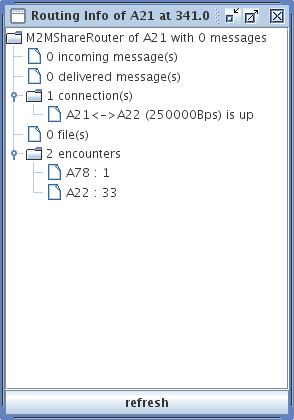
\includegraphics[scale=0.6]{6-implementazione/img/Routing-Info.png}
    \caption{An example of window with a detailed view of a node state}    
    \label{implRouting-Info}
  \end{center}
\end{figure}

\subsection{Reports}
\label{descrReports}
A fundamental feature related to simulations is the ability to gather data from different aspects of the simulated world, like positions of nodes, communications, data transfers and so on. To achieve this goal in the ONE are used some special modules named \textit{Report Generators} which works with some related Listeners to catch the interested events in the simulated scenario and save them to some report files.
The main objectives of our simulations was to gather information about the efficiency of delegations and file division strategies, and to do so we collected data about several aspects for every simulation. We will now describe the report modules created to the gathering of data during the simulations, specifying the type and mode of data collection used.

\paragraph{FileGatheringLog}
The first report module is a log report module, that stores the selected events in a list, saving them to file, one event per line. This module is responsible for listening for the following events:
\begin{itemize}
\item \textbf{VirtualFile creation:} a new \textit{VirtualFile} has been created due to the execution of a \textit{FileRequest} in a node. It emulates a user requesting a new file to be found and downloaded.
\item \textbf{DTNPendingDownload creation:} a new \textit{DTNPendingDownload} has been created in a servant peer thanks to the delegation of a task from a client node.
\item \textbf{DTNPendingDownload completion:} a \textit{DTNPendingDownload} has been completed in a servant peer (the servant has downloaded all the requested file intervals subject of the delegated task). Consequently a \textit{DTNDownloadFWD} has been created and queued in the servant.
\item \textbf{DTNPendingDownload expiration:} a \textit{DTNPendingDownload} has expired in a servant peer before being completed (the servant has not downloaded all the requested file intervals subject of the delegated task).
\item \textbf{DTNDownloadFWD expiration:} a \textit{DTNDownloadFWD} has expired in a servant peer before being completed (the servant has not forwarded all the requested file intervals subject of the delegated task to the requester node).
\item \textbf{DTNDownloadFWD completion:} a \textit{DTNDownloadFWD} has been completed in a servant peer (the servant has forwarded all the requested file intervals subject of the delegated task to the requester node).
\end{itemize}

Every event is saved in the following format:
\begin{center}
\textit{Sim\_time	event\_description	event\_details}
\end{center}
The following are some examples:

\begin{center}
\textbf{15538.0000	PendingDownload	A32 to E476}
\end{center}
Refers to the task delegation from the node A32 to the node E467, 15538 seconds after the beginning of the simulation.
\\

\begin{center}
\textbf{38559.5000 PendingDownload completed in F630 (317200191 requested by A32)}
\end{center}
Refers to the completion of the \textit{DTNPendingDownload} in the servant node F630 at time 38559.5. It was delegated by the node A32 and the id of the searched file was \textit{317200191}
\\

\begin{center}
\textbf{213738.0000	DownloadFWD expired in F523 (317200191 requested by A32)}
\end{center}
Refers to the expiration of the \textit{DownloadFWD} in the servant node F523 at time 213738. It was delegated by the node A32 and the id of the searched file was \textit{317200191}
\\

\paragraph{DataTransferLog}
\textit{DataTransferLog} module is another log module, which keeps track of events regarding data transfer between nodes in the simulation. These can occur during the execution of several activities:
\begin{itemize}
\item \textbf{VirtualFile:} when the requester peer is in range with a node carrying the searched file, and the data transfer take place. Multiple data transfer events can be generated, if there are several peers with the searched file in range.
\item \textbf{DTNPendingDownload:} when a servant peer downloads, from a node carrying the searched file, some requested intervals contained in the delegated task.
\item \textbf{DTNDownloadFWD:} when a servant peer forwards the result of a delegated \textit{DTNPendingDownload} to the client peer.
\end{itemize}
Data transfer events are saved in the following format:
\begin{center}
\textit{Sim\_time	from\_address	to\_address	data\_transferred (in bytes)}
\end{center}
e.g.
\begin{center}
\textbf{98829.0000	G714	A17	2750001}
\end{center}
Refers to the data transfer from node G714 to node A17, 98829 seconds after the start of the simulation. 2750001 bytes have been transferred in this event.
\\

\paragraph{FileGatheringReport}
\textit{FileGatheringReport} module is the most important report module used during our simulations, because it summarizes all key aspects of a single simulation. In detail, these are the values tracked by this module:
\begin{itemize}
\item \textbf{Total data:}	the total amount of data traffic exchanged between servant peers trying to satisfy a delegated task, file possessor peers and the data forwarding quantity toward the requester node.
\item \textbf{VirtualFile created:}	number of \textit{VirtualFile} task created during the simulation
\item \textbf{VirtualFile delegated:} how many times a task has been delegated to a servant peer
\item \textbf{PendingDownloads completed:} how many of the delegated tasks have been completed i.e. how many times the servant peer has been able to locate and download all the data intervals requested in the \textit{DTNPendingDownload} 
\item \textbf{PendingDownloads expired:} how many of the delegated tasks expired before the servant peer being able to find and download all the data intervals requested in the \textit{DTNPendingDownload} 
\item \textbf{DownloadFWDs expired:} how many \textit{DownloadFWDs} expired i.e. the servant peer downloaded all the data intervals requested in the \textit{DTNPendingDownload} but it was not able to forward them to the requester peer before the task expiration
\item \textbf{DownloadFWDs returned:} how many \textit{DownloadFWDs} has been forwarded correctly to the requester peer
\item \textbf{VirtualFile completed:} how many of the created \textit{VirtualFile} has been completed
\item \textbf{First VirtualFile satisfied:}	the time (in seconds) passed from the file request creation before the \textit{VirtualFile} has been completed
\item \textbf{Simulated time:} the simulated duration (in seconds) of the simulation
\item \textbf{Simulation time:}	the real duration of the simulation (in seconds)
\end{itemize}
Saving all these values for every simulation is useful in order to make later analysis such as averages, minimum and maximum values and to find the best or worst case for a large number of simulations.

\paragraph{M2MShareMapCoverageReport}
In order to evaluate the achieved explored area using different delegation strategies we implement the \textit{M2MShareMapCoverageReport}. This module divides the simulated map in squares with size of 10 x 10 meters and counts how many times each square has been visited during the simulation. When a node moves, the module saves its position by adding 1 to the value of the related square. The report is configurable, in order to save only movements related to nodes employing different delegation strategies:
\begin{itemize}
\item the node with the initial file request issued by the user
\item nodes acting as servants, i.e. nodes with delegated tasks received
\item all nodes in the simulation
\end{itemize}
The reason we decided to save all nodes movements, in some simulations, is to obtain a \textit{control set} to evaluate the maximum area that can be explored using certain parameters. By doing so for a high number of simulations we see which parts of the map can be explored (streets, buildings, parks) and which are not (like rivers, the sea or places not reachable with nodes movement).

%
%\paragraph{DelegationGraphvizReport}
%The last report module implemented for our simulation is a module responsible for the creation of reports describing the delegation history of the simulation using a Graphwiz graph. These graphs are described using the DOT language and can be displayed using the \textit{Graphwiz Graph Visualization Software}\footnote{http://www.graphviz.org/}. These graphs are useful to get a visual feedback about the delegations of tasks done and the status of that tasks, especially in case of multi-hop delegations. For every peer involved in delegations can be seen:
%\begin{itemize}
%\item if it receive the delegation (obviously)
%\item if it complete the delegated task
%\item if it forwarded back the result of the delegated task
%\end{itemize}
%In figure \ref{graph-example}
%\figuremacro{graph-example}{Graphviz graph example}{An example of graph generated using the output of DelegationGraphvizReport module}{}


\section{M2MShare Implementation}
In this section we describe the implementation of modules composing M2MShare into the ONE simulator. As said earlier in Section \ref{simulatore}, every routing protocol is an extension of a common superclass named \textit{MessageRouter} and, according to the the ONE philosophy, a new routing module can be inserted extending that class and it can be consequently used in configuration time to set the routing behaviour of nodes.
\\

M2MShare implementation consists in the main class extending \textit{MessageRouter}, named \textit{M2MShareRouter}, and several other classes contained in the package \textit{routing.m2mShare}.

\paragraph{M2MShareRouter}
As mentioned earlier, this is the main class of M2MShare implementation. Its first responsibility is to load the related settings as set in configuration files (see Section \ref{configurazioneONE}) and to initialize all the modules needed for the execution of the protocol. These entities will be described later and are responsible of the different aspects of the protocol. Values used to initialize the settings are read from configuration files and all are included in the settings namespace \textit{M2MShareRouter}. Every parameter has a default value, used in case nothing is not specified in any configuration file. Here the available parameters are shown and, shown in brackets, the relative default value:
\begin{itemize}
\item \textbf{M2MShareRouter.frequencyThreshold [2]} indicates the minimum number of encounters needed to elect a peer as servant and consequently delegate a task to it 
\item \textbf{M2MShareRouter.scanFrequency [10]} indicates how many seconds the \textit{PresenceCollector} must to wait between one scan and the next
\item \textbf{M2MShareRouter.delegationType [1]} indicates the type of delegation strategy used. It accepts three values:
\begin{itemize}
\item \textbf{0:} do not use delegation and file exchange is initiated only when a peer holding the requested data file is found in the reach area 
\item \textbf{1:} use the M2MShare technique where unaccomplished tasks are delegated only to peers which exceed the \textit{frequencyThreshold} value
\item \textbf{2:} use the trivial technique where unaccomplished tasks are delegated to each encountered peer
\end{itemize}
\item \textbf{M2MShareRouter.fileDivisionType [1]} indicates the type of file division strategy used. It accepts three values:
\begin{itemize}
\item \textbf{0:} for every file transfer is requested the entire file
\item \textbf{1:} use the M2MShare technique to choose the initial download point in the requested file
\item \textbf{2:} randomly choose the initial download point in the requested file
\end{itemize}
\item \textbf{M2MShareRouter.useBroadcastModule [true]} used to enable/disable the broadcast module. Could be useful to speed-up simulations, at the cost of a loss of precision
\item \textbf{M2MShareRouter.delegationDepth [1]} indicates the maximum number of delegation hops can be used for delegations, starting from the initial requester
\item \textbf{M2MShareRouter.stopOnFirstFileRequestSatisfied [false]} used to make the simulation stop when the first File Request has been satisfied. Can be useful in simulations in which we are not interested in what happens after the File Request is satisfied
\end{itemize}

%The class \textit{M2MShareRouter} also extends the superclass \textit{MessageRouter} and doing so it override the main method of this class: \textit{update()}. As said in Section \ref{esecuzioneONE}, that method is called one time for every simulated time interval, after the update of movement and connections of the node. In \textit{M2MShareRouter} the only action executed in \textit{update()} is to call the method \textit{runUpdate()} in module \textit{Scheduler}, described in section \ref{schedulerImplementazione}.

\paragraph{PresenceCollector}
The module \textit{PresenceCollector} is responsible for gathering information about in-reach area devices and to track encounters between other nodes to realize the election strategy selected for the current node in the simulation. Encounters data is gathered scanning for in-reach devices with a fixed frequency. When another node exceeds a value named \textit{Frequency Threshold}, it can be elected as a servant and receive unaccomplished tasks as delegations from the current node. Encounters data is saved in a structure called \textit{Servant List} which uses a replacement policy to manage peer slots in the list. If a peer has been encountered for a period greater than a value, called \textit{Probation Window}, without being elected as servant, its slot is freed to give other peers the opportunity to be elected as servants. \textit{PresenceCollector} also includes a tuning algorithm which adapts \textit{Frequency Threshold} and \textit{Probation Window} values at the beginning of every simulated day, according to what observed during the previous day.


\paragraph{Activities}
A single node in M2MShare system can execute several kinds of tasks. In our implementation, each of them is an implementation of interface \textit{DTNActivity} and characterizes one task type respect to another for what concerns their execution. 
\\

In a \textit{VirtualFile} task type, the execution is focused on searching in-reach devices for the file the user asks to find and download. A VirtualFile includes an IntervalMap used to store those file pieces that are still missing. When a VirtualFile task is completed, a new DTNFile is created and saved in the node's file system. 
\\

A VirtualFile can be delegated to a servant peer. When a servant node receives a delegated task, it creates and queues a \textit{DTNPendingDownload} activity. In its execution, the servant node searches in-reach devices for requested intervals of the file described in the delegated task. When a DTNPendingDownload task is completed, the servant node creates end schedules a \textit{DTNForward} task for execution.
\\

In this task's execution, the servant node looks for the client node that delegated it the VirtualFile task. When this node is found, the servant node notifies that it is ready to forward the output of the DTNPendingDownload task. The client can request all or only a subset of intervals the servant downloaded.
\\

Tasks active in servant nodes (DTNPendingDownload and DTNForward) have a TTL value, calculated using client's Probation Window value. When this value is exceeded, the task is deleted from queues and never again scheduled for execution.
\\

With our addition to M2MShare first version, a task can be delegated with more than one hop. To do so we allow M2MShareRouter to delegate also incomplete DTNPendingDownload activities. The result of this delegation, in servant peer, is the creation of a new DTNPendingDownload task. A delegation history list is included in every delegated task. When this second-level task is completed, a new DTNForward task is created in the servant peer. Its execution consists in returning the output of the second-level delegation to one of the nodes in delegation history list. This allows to return the output to the initial requester node faster than returning it following the inverse order of delegation history list.
\\

To avoid generating an high number of delegations, we set a trial period before a servant node delegate again a pending task. It waits one day and during this period it tries to complete the task by itself. If the task is still incomplete after one day, the node proceeds to delegate it for another hop. The maximum number of hops for each delegation is configurable for every simulation. To avoid delegation cycles, we implemented an anti-cycle system similar to the one used in AODV \cite{aodv} which prevents delegating a task to a node that is already acting as servant for it. 

\paragraph{File Division Strategies}
To evaluate the efficiency of M2MShare file division strategy, we implemented a \textit{IntervalMap} according to the one described in Section \ref{descrFileDivisionStrategy}. This structure includes not yet downloaded intervals for a file and is used by our system's Activities to implement the adopted file division strategy. Its behaviour can be set through configuration files for every simulation. This allow emulations of different file division strategies and comparing their efficiency in several simulations:
\begin{itemize}
\item \textbf{M2MShare:} the strategy with dynamic starting point, described in Section \ref{descrFileDivisionStrategy}
\item \textbf{iM:} where each file transfer starts from the beginning of the file
\item \textbf{rM:} where each file transfer starts from a random point within the file
\end{itemize}


\paragraph{Data Transfer}
To emulate data transfers between nodes in the simulated network, we implement a entity named \textit{Communicator}. This entity is used by Activities to emulate the downloading of pieces of files from a file possessor, or the forwarding of a pending task's result to a client node. There is no 1-1 relation between Communicators and Activities. A task can use more than one Communicator when try to simultaneously download pieces of the same file from different sources within communication range. Communicator behaviour is related to the adopted file division strategy, as it influences the starting point of file transfers. Using Communicators allows us to emulate data transfers only when a connection between two nodes is available and to notify information about transfers to related report modules.

%\paragraph{Scheduler}
%\label{schedulerImplementazione}
%\paragraph{Executor}
%\paragraph{Communicator}
%
%\paragraph{BroadcastModule}
 
\section{Analysis}
To evaluate M2Mshare efficiency we need to analyse its performance compared with other strategies or with different versions of M2MShare, as in multi-hop simulations. To do so we repeat each simulation several times changing the random module generators seeds. We do so to achieve results independent from nodes movement and the starting point. For each simulation we save some report files, generated using report modules described in Section \ref{descrReports}. Several analyses have been made over these reports using a set of classes we implemented for this purpose. 
\\

Repeating each simulation with different strategies we are able to compare their performance related to several values. Using our report and analysis modules, for each single simulation we are able to evaluate:
\begin{itemize}
\item number of File Requests created
\item how many tasks have been delegated during the simulation
\item how many delegated tasks have been completed
\item how many delegated tasks expired before completion
\item how many delegated tasks have been completed but expired before the result was forwarded to the requester node
\item number of File Request satisfied
\item after how much time a File Request has been satisfied
\item the length of simulated time
\item the length of the simulation (in real time)
\end{itemize} 

For each set of simulations repeated changing random generators seeds, we are able to evaluate 
\begin{itemize}
\item minimum value
\item maximum value
\item average value
\end{itemize} 
related to each of the parameters above.
 
% ---------------------------------------------------------------------------
%: ----------------------- end of thesis sub-document ------------------------
% ---------------------------------------------------------------------------


% this file is called up by thesis.tex
% content in this file will be fed into the main document

%: ----------------------- name of chapter  -------------------------
\chapter{Simulations and results}\label{simulazione} % top level followed by section, subsection


%: ----------------------- paths to graphics ------------------------

% change according to folder and file names
%\graphicspath{{2-Consorzi/images/}}


%: ----------------------- contents from here ------------------------
In previous chapters we focused on the concepts, related technologies and implementation realized of the protocol, M2MShare, subject of the study of this thesis. In this section we describe the simulations executed and analysis with relative results. For every type of analysis we describe the related simulations, the configuration of the simulated world and the other protocols compared to our M2MShare. Finally, for every analysis, we show the results graphically with a textual interpretation.
\\

Before proceeding further, we introduce the reader to the adopted terminology and some "must know" configuration parameters:
\begin{itemize}
\item \textit{Population}: refers to the number of nodes in the simulation which emulate people operating M2MShare. This number does not include nodes which emulate public transport, like buses or trams. People are distributed in districts of the map, described in Section \ref{mappaONE}.

\item \textit{File size}: refers to the size of the data file the user is looking for in the simulation 

\item \textit{File popularity}: refers to how many copies of the data file the user is looking for in the simulation are present at the beginning of the simulation. It is specified using the percentage of nodes which have the file at the beginning of the simulation. Nodes initially carrying the file are randomly chosen, using the DTNFileGenerator described in Section \ref{fileGeneratorImplementazione}.

\item \textit{File distribution}: refers to how files are distributed among the population at the beginning of the simulation. Nodes initially carrying the file can be uniformly chosen from among all the active nodes or in a subset of them.

\item \textit{Delegation Type}: refers to the type of delegation used in the group of simulations. It can be of three types:
\begin{itemize}
\item \textbf{No\_delegation:} do not use delegation and file exchange is initiated only when a peer holding the requested data file is found in reach area 
\item \textbf{M2MShare:} uses the M2MShare technique where missing tasks are delegated only to peers which exceed the \textit{frequencyThreshold} value
\item \textbf{Delegation\_to\_all:} use the trivial technique where missing tasks are delegated to each encountered peer
\end{itemize}

\item \textit{Delegation Depth}: how many times a delegated task can be re-delegate to other peers.

\item \textit{Multi-hop delegation probability (MhDP)}: the probability that a servant peer would delegate again a pending incomplete task. This is specified only for simulations with multi-hop delegation.

\item \textit{File Division Strategy}: refers to the type of file division strategy used during file transfer between nodes. It can be of three types:
\begin{itemize}
\item \textbf{M2MShare:} use the M2MShare technique to choose the initial download point in the requested file
\item \textbf{iM:} for every file transfer is requested the entire file
\item \textbf{rM:} randomly choose the initial download point in the requested file
\end{itemize}

\item \textit{Nr. of simulations}: how many times the simulation has been repeated with different movement and file generation seeds.

\item \textit{Simulated time}: the simulated length of simulations

\end{itemize}


\section{Simulations Scenario}
In this section we describe the scenario implemented to evaluate the performance of M2MShare with the ONE simulator. The following are the default values used to initialize our simulations, that is if changes are not described in sections relative to a single simulation, these are the values used.
\\

For our simulations we the map of Helsinki city centre and surrounding districts included in the ONE. The map has a size of about 8000 x 7000 m$^{2}$ and is described in Section \ref{mappaONE}. 


To increase the trustworthiness of the experimental outcome we have included realistic day-by-day node movements through the Working Day Movement (WDM) model, described in Section \ref{descrWDM}. As anticipated, this model is able to represent both the unpredictability of certain movements of users and the routine of other movements such as, for instance, the daily trip from home to work. This provides a good approximation of inter-contact times and contact durations, providing the flexibility for configuring real life test scenarios.
\\

We use the same configuration parameters described in \cite{articoloWdm}, to initialize the movement model. Nodes population is variable during the simulations but the map is always divided in districts, with overlapping between them. There are several bus routes, one for every district and every node can use a bus of the route belonging to the same district of the node. When a node is walking, the speed is set between 0.8 and 1.4 m/s and for buses between 7 and 10 m/s, with a 10 - 30 s waiting at each stop. Half of all the nodes were set to travel by car and the speed of cars is set to 20 m/s to make it a faster way to move between locations. 
\\

To emulate differences in people's lifestyles, especially in morning wake up times, the differences in schedules of nodes were drawn from a normal distribution with a standard deviation of 7200 s emulating a situation where about 68\% of the population leaves home between 7 and 11 in the morning. Every node has a probability of 0.5 of doing some activity in the evening, after work, with groups size variable between 1 and 3 nodes. The working day length is set to 28800 s (8 hours), which is a value common to a large number of jobs, and the pause times inside the office is drawn from a Pareto distribution with coefficient 0.5 and minimum value 10 s. The office size is set to a $100 m x 100 m$ square, to compensate for the lack of floors, walls and other furniture. Finally the communication range of mobile devices is set to 10 m, which is common for most Bluetooth devices.
\\

We repeat each of the simulation scenarios several times in order to achieve more accurate results, independent of the initial positioning of the requester peer in search for that particular data file and independent of the initial positioning of the searched file copies. Each scenario is run using a different random seeds to initialize the movement model and for every seed the simulation is repeated using the compared protocols.

\newpage
\section{Single-hop delegation efficiency}
\label{analisiDelegationEfficiency}
\begin{table}[h]
\begin{center}
\begin{tabular}{|l|r|}
\hline
\bfseries Population & 1000 \\
\hline
\bfseries File size & 3.0 MB \\
\hline
\bfseries File popularity & 5\% \\
\hline
\bfseries File distribution & Uniformly distributed \\
\hline
\bfseries Delegation type & No\_delegation, M2MShare, Delegation\_to\_all \\
\hline
\bfseries Delegation depth & 1 \\
\hline
\bfseries File Division Strategy & M2MShare \\
\hline
\bfseries Nr. of simulations & 40 x 3\\
\hline
\bfseries Simulated time & One week \\
\hline
\end{tabular}
\end{center}
\caption{Simulations settings for evaluation of delegation efficiency\label{tab:settingsIniziali}}
\end{table}
In this analysis we evaluate the efficiency in using delegation versus not using it.  \tablename~\ref{tab:settingsIniziali} shows the settings used for these simulations and we can see that we compare the efficiency of our system (M2MShare) employing one-hop delegations against two other systems using different strategies:
\begin{itemize}
\item \textit{No\_delegation:} system which does not employ delegations and file exchange is initiated only when a peer holding the requested data file is found in reach area of file requester.
\item \textit{Delegation\_to\_all:} system employing delegations but instead employs the trivial technique where missing tasks are delegated to each encountered peer.
\end{itemize}

The metric we study is the found time ($F_{t}$) for a generic data file which is the time interval between the first delegation made and the time an output return for that specific file is
received. If no delegations are made and the first file request is satisfied by a direct file possessor the $F_{t}$ is equal to zero. For each of the above scenarios we also measure the:
\begin{itemize}
\item number of delegations used: representing the number of tasks the requester peer has delegated for that particular data download;
\item percentage of completed task: representing the number of delegated tasks completed (output returned) over all delegated tasks;
\item total data transferred: referring to the quantity of data traffic exchanged between servant peers trying to satisfy a delegated task, file possessor peers and the quantity of data forwarded towards the requester node.
\end{itemize}

\begin{figure}[!htbp]
\centering
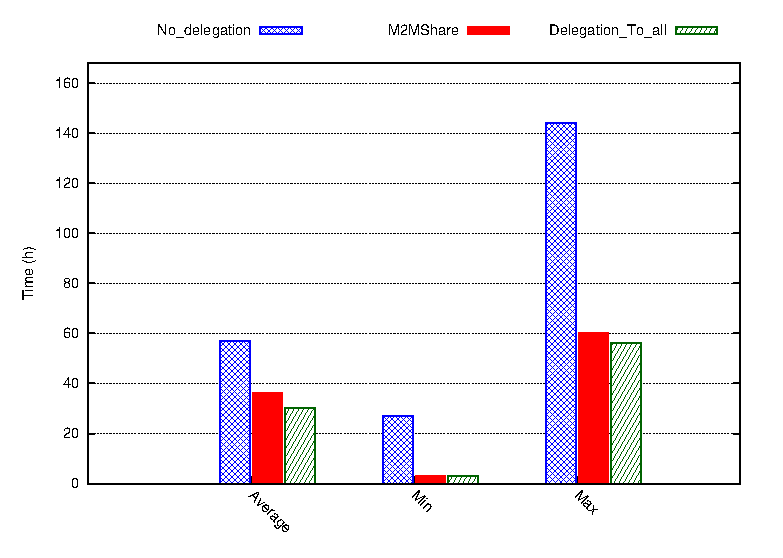
\includegraphics{grafici/tempi.eps}
\caption{Average, min. max found time employed by each strategy in finding the required data file.}
\label{graficoTempiVF}
\end{figure}

\begin{figure}[!htbp]
\centering
%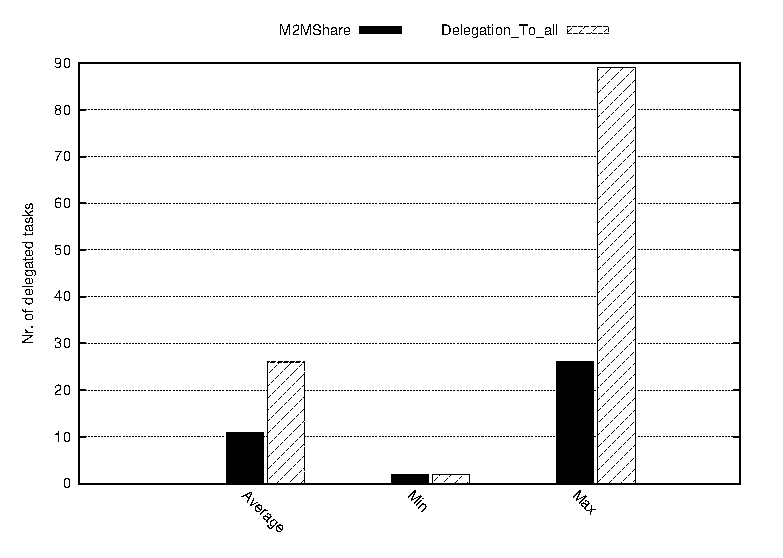
\includegraphics[scale=0.7]{grafici/delegheFatte.eps}
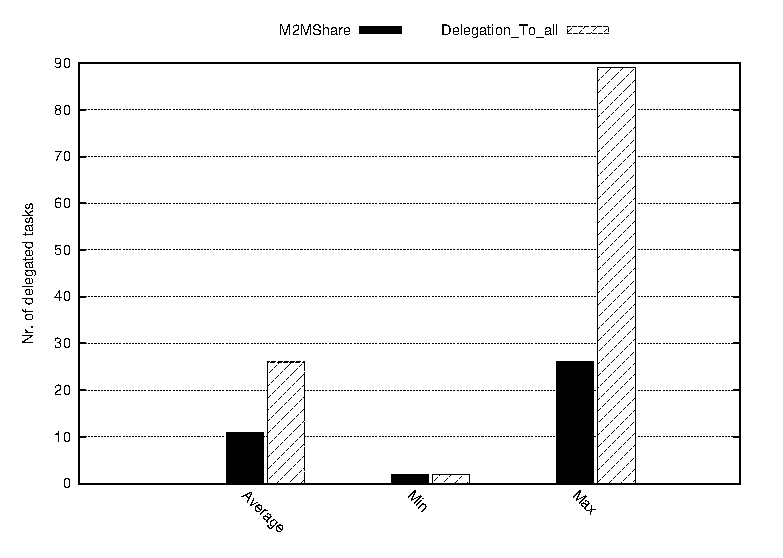
\includegraphics{grafici/delegheFatte.eps}
\caption{Average, min, max number of delegations employed by each delegation strategy.}
\label{graficoNumeroDeleghe}
\end{figure}

%\begin{figure}[ht]
%\begin{minipage}[b]{0.45\linewidth}
%\centering
%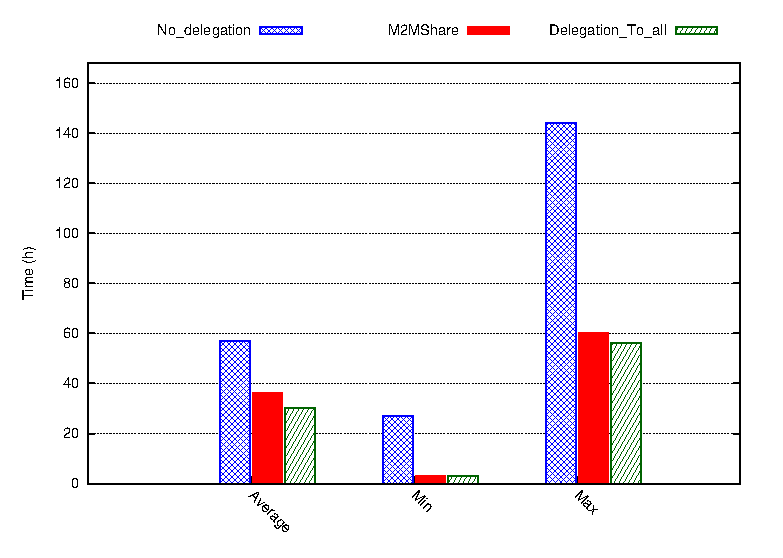
\includegraphics[scale=0.45]{grafici/tempi.eps}
%\caption{Average, min. max found time employed by each strategy in finding the required data file.}
%\label{graficoTempiVF}
%\end{minipage}
%\hspace{0.5cm}
%\begin{minipage}[b]{0.45\linewidth}
%\centering
%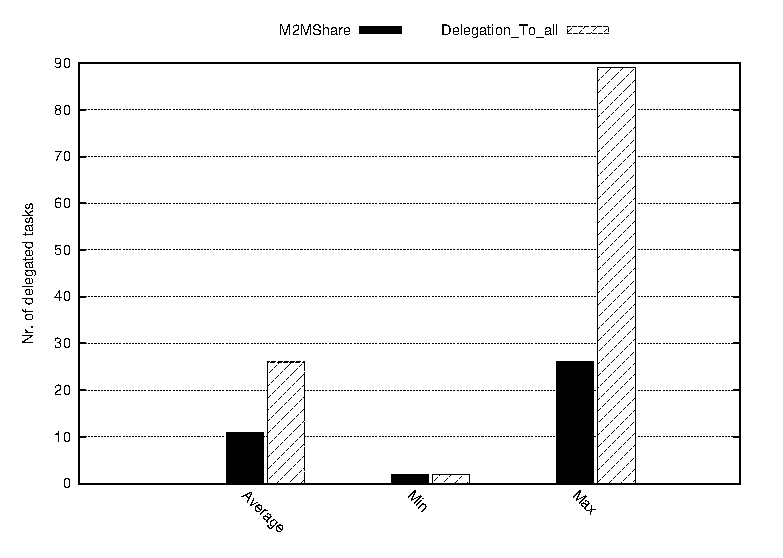
\includegraphics[scale=0.45]{grafici/delegheFatte.eps}
%\caption{Average, min, max number of delegations employed by each delegation strategy.}
%\label{graficoNumeroDeleghe}
%\end{minipage}
%\end{figure}


In \figurename~\ref{graficoTempiVF} it is possible to see the advantage, in terms of found time, in using the delegation technique instead of not using it. The two systems employing delegations find the required file in less time in each simulation run at the expense of higher overhead in terms of bandwidth due to delegations. The system employing delegations to all encountered peers obtains a better result on average, but at the cost of a higher number of delegated tasks (\figurename~\ref{graficoNumeroDeleghe}). A higher number of delegated tasks imply more bandwidth used for searching the data file and potentially retrieving (if found) and forwarding it toward the requester.
\\

%\begin{figure}[ht]
%\centering
%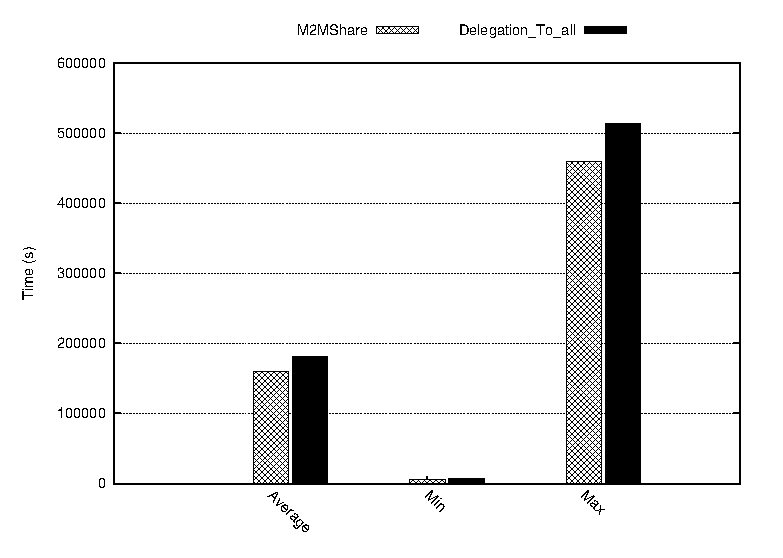
\includegraphics[scale=0.7]{grafici/tempiRitornoDeleghe.eps}
%\caption{Average, min, max output return time for systems using task delegations.}
%\label{graficoRitornoMedioDeleghe}
%\end{figure}

\figurename~\ref{graficoNumeroDeleghe} makes a comparison between the two systems employing delegations by showing the number of overall employed task delegations till file download or simulation time expires. It is easy to see that M2MShare uses fewer delegations while achieving a higher percentage of completed delegated tasks (\figurename~\ref{graficoPercDelegheRitornate}). This outcome is due to a conservative delegation strategy employed by M2MShare in delegating unsatisfied, unaccomplished tasks only to frequently encountered peers (servants). Since we do not have any means for evaluating the ability of one servant to satisfy a file request what we do is delegate to the encountered peers that can be expected to be encountered again in the future. The Delegation\_to\_all strategy also contributes to higher overhead due to completed tasks, ready to be returned towards the requester that unfortunately expire and are discarded before having the chance of encountering the data file requester. \\
%It is also possible to see in \figurename~\ref{graficoRitornoMedioDeleghe} that in M2MShare it takes less time, on average, for a servant to return the output of a delegated task which has been completed, i.e. not expired, to the requester node.
%\\

%\begin{figure}[htbp]
%\begin{minipage}[b]{0.5\linewidth}
%\centering
%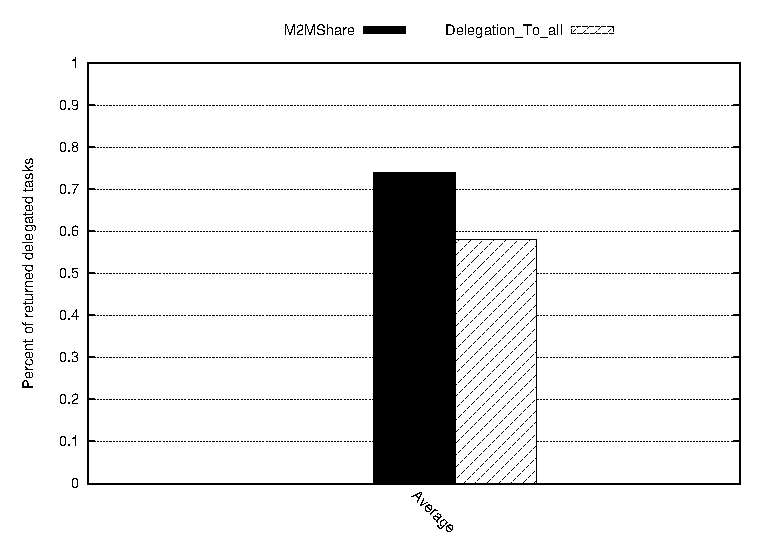
\includegraphics[scale=0.5]{grafici/percDeleghe.eps}
%\caption{Percentage of completed previously delegated tasks against the number of overall delegations employed.}
%\label{graficoPercDelegheRitornate}
%\end{minipage}
%\hspace{0.5cm}
%\begin{minipage}[b]{0.5\linewidth}
%\centering
%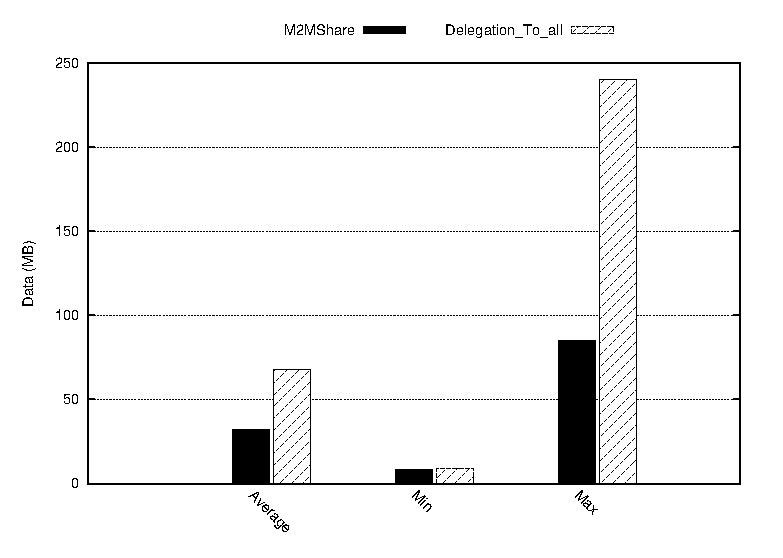
\includegraphics[scale=0.5]{grafici/data.eps}
%\caption{Average, min, max transferred data amount employed in each delegations technique.}
%\label{graficoDataDiverseDel}
%\end{minipage}
%\end{figure}

\begin{figure}[htbp]
\centering
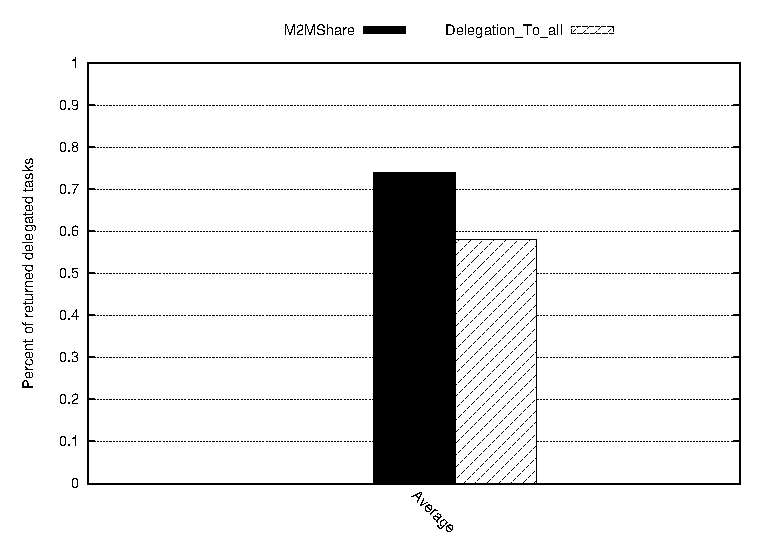
\includegraphics{grafici/percDeleghe.eps}
\caption{Percentage of completed previously delegated tasks against the number of overall delegations employed.}
\label{graficoPercDelegheRitornate}
\end{figure}

\begin{figure}[htbp]
\centering
%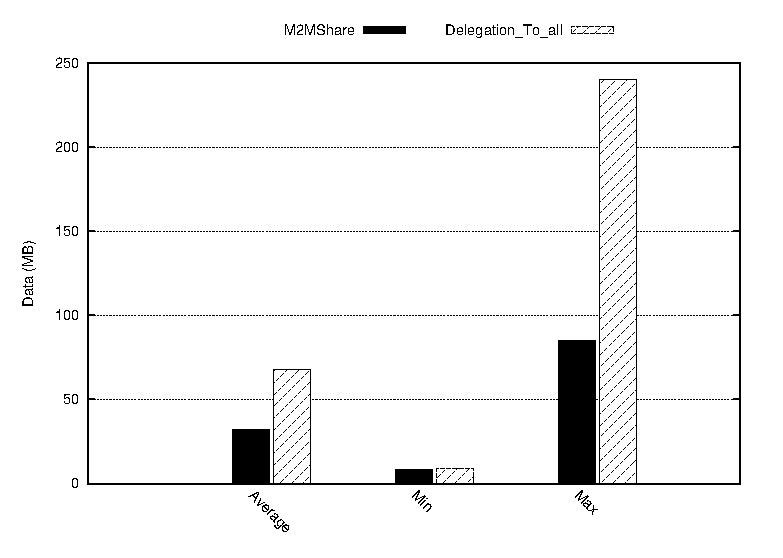
\includegraphics[scale=0.7]{grafici/data.eps}
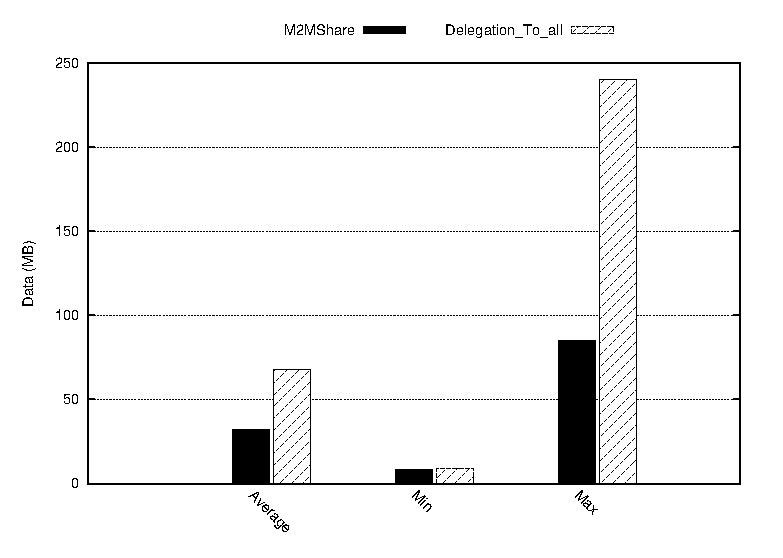
\includegraphics{grafici/data.eps}
\caption{Average, min, max transferred data amount employed in each delegations technique.}
\label{graficoDataDiverseDel}
\end{figure}


\figurename~\ref{graficoDataDiverseDel} shows the comparison between M2MShare and Delegation\_to\_all strategies in terms of transferred data quantities until file download or simulation time ends. It is straightforward to notice the higher overhead in terms of data transmissions introduced by delegating to all encountered peers whether M2MShare reduces the exchanged data quantity while still achieving the goal of acquiring the requested file. From the above results it is obvious that the delegation strategy serves its purpose by extending a peer reach area to other mobile disconnected networks where data content might be available therefore reducing the found time of a desired content.
Although this strategy introduces an overhead in terms of bandwidth usage, computation and power consumption we control these side effects by delegating only to frequently encountered peers whom are expected to be encountered again in the future.



\newpage 
\subsection{Delegation efficiency with variable file popularity}

\begin{table}[h]
\begin{center}
\begin{tabular}{|l|r|}
\hline
\bfseries Population & 1000 \\
\hline
\bfseries File size & 3.0 MB \\
\hline
\bfseries File popularity & 5\%, 10\%, 15\%, 20\%, 25\%, 30\%, 35\%, 40\% \\
\hline
\bfseries File distribution & Uniformly distributed \\
\hline
\bfseries Delegation type & No\_delegation, M2MShare, Delegation\_to\_all \\
\hline
\bfseries Delegation depth & 1 \\
\hline
\bfseries File Division Strategy & M2MShare \\
\hline
\bfseries Nr. of simulations & 40 x 8 x 3\\
\hline
\bfseries Simulated time & One week \\
\hline
\end{tabular}
\end{center}
\caption{Simulations settings for evaluation of delegation efficiency with variable file popularity\label{tab:settingsDiversaFilePop}}
\end{table}
In previous analysis we show the advantage, in terms of found time of the searched file, using M2MShare delegation strategy against avoiding using delegation or delegating unaccomplished tasks to every node met. The confrontation was made using a constant number of copies of the searched multimedia file uniformly distributed between all nodes in the simulation, i.e. 50 copies. The current analysis wants to show the difference in performance using the three delegation strategies changing the initial file popularity of the searched file. To this aim, in these simulations we change the File popularity (Fp) of the multimedia file keeping constant the number of total nodes (N). Simulations settings are shown in \tablename~\ref{tab:settingsDiversaFilePop}.

We change the File Popularity (Fp) value, from 5\% (50 copies) to 40\% (400 copies). When the Fp is low (with Fp $\geq 5\%$) the system which does not use delegation is not able to find any piece of the file during the simulation time. We have indicated this in the chart by assigning to Ftavg a value of 48 h. With higher values of Fp, the first protocol is able to find the file thanks to the higher popularity of the requested file, but it takes more time than M2MShare and Delegation\_to\_all. Finally, with the highest values of Fp the performances of the three compared systems becomes very similar. 


\begin{figure}[htbp]
\centering%
\subfigure%
{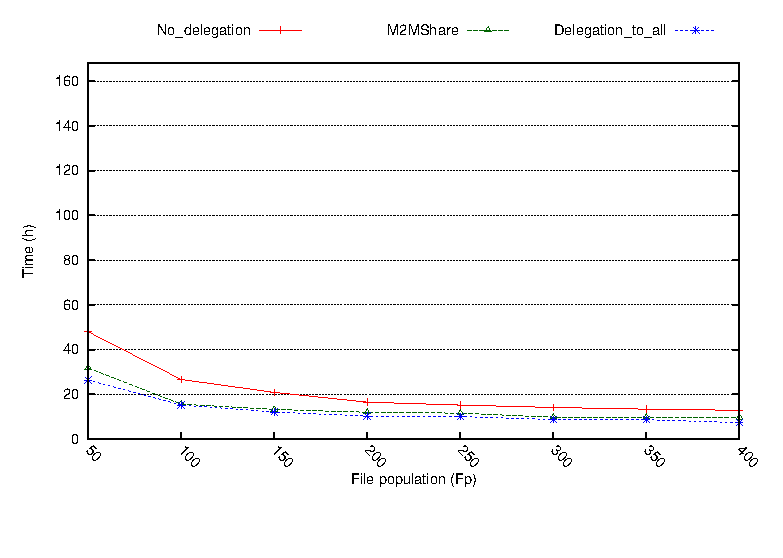
\includegraphics{grafici/tempiVFDiversaPop.eps}}\qquad\qquad
\subfigure%
{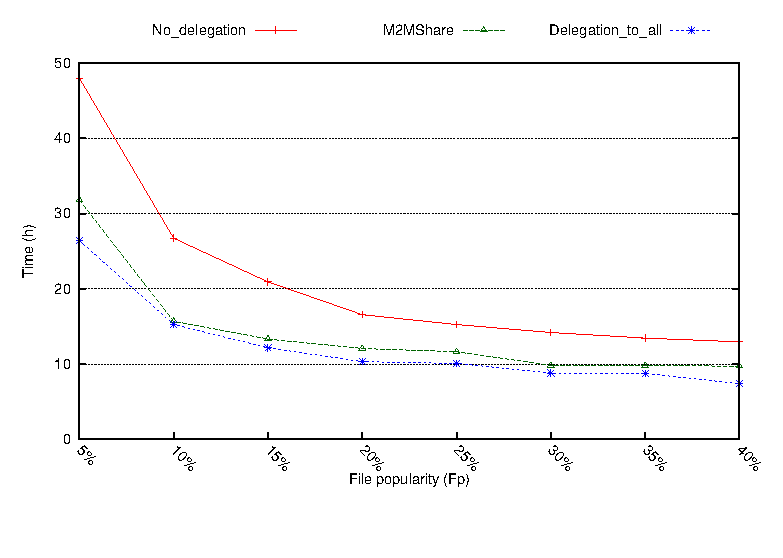
\includegraphics{grafici/tempiVFDiversaPop_zoom.eps}}
\caption{Average found time with variable file popularity\label{graficoPopVariabile}}
\end{figure}


\newpage
\subsection{Delegation efficiency with variable nodes population}
\begin{table}[h]
\begin{center}
\begin{tabular}{|l|r|}
\hline
\bfseries Population & 100, 200, 400, 600, 800, 1000 \\
\hline
\bfseries File size & 3.0 MB \\
\hline
\bfseries File popularity & 5\%, 10\%, 50\% \\
\hline
\bfseries File distribution & Uniformly distributed \\
\hline
\bfseries Delegation type & No\_delegation, M2MShare, Delegation\_to\_all \\
\hline
\bfseries Delegation depth & 1 \\
\hline
\bfseries File Division Strategy & M2MShare \\
\hline
\bfseries Nr. of simulations & 40 x 6 x 3 x 3\\
\hline
\bfseries Simulated time & One week \\
\hline
\end{tabular}
\end{center}
\caption{Simulations settings for evaluation of delegation efficiency with variable nodes population and file popularity\label{tab:settingsDiversoNePop}}
\end{table}

In previous analysis we considered as constant the number of nodes emulating people using M2MShare on their devices. As we can see in \tablename~\ref{tab:settingsDiversoNePop}, in the current analysis we changed the total nodes population of the simulations and the searched file popularity, observing how this affects the performance of compared systems.\\

In the first scenario (\figurename~\ref{graficiTempiVF_Fp5}) we consider Fp = 5\%. The protocol not employing delegations (black line in the chart) is not able to find any piece of the file during the simulation time when the considered nodes in the scenario are equal or less than 400. We have indicated this in the chart by assigning to Ftavg a value of 48 h. This is due to the trivial strategy employed by the protocol and to the sparse environment. Even when able to find some node possessing the file (with N $\geq 600$), the time needed results bigger than using a strategy implementing delegations. Clearly, when increasing the file population (Fp), even the number of nodes in the population that posses the data file increases; as a result, the time to retrieve the file decreases for all solutions. A similar result is achieved also when considering a wider popularity for the required multimedia file (Fp = 10\%, in \figurename~\ref{graficiTempiVF_Fp10}). However, in this case, the higher popularity of the requested file helps both solutions in finding the file possessor with a smaller Ftavg than in the previous scenario.  Finally, in \figurename~\ref{graficiTempiVF_Fp50}, the performances of the compared solutions are very similar. This is due to the high file popularity among nodes (Fp = 50\%): the chances of eventually finding a file possessor in a short time are clearly much higher.

%\begin{figure}[ht]
%\begin{minipage}[b]{0.5\linewidth}
%\centering
%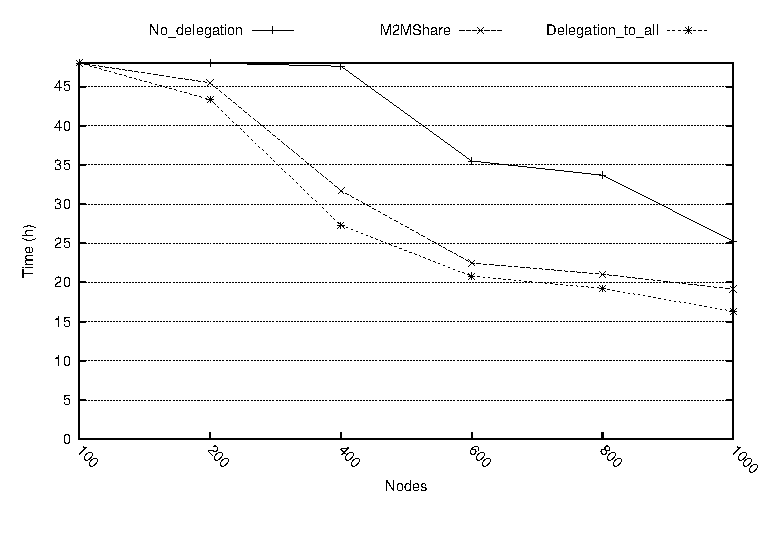
\includegraphics[scale=0.5]{grafici/tempiVF_Fp5.eps}
%\caption{Average found time with $Fp = 5\%$}
%\label{graficiTempiVF_Fp5}
%\end{minipage}
%\hspace{0.5cm}
%\begin{minipage}[b]{0.5\linewidth}
%\centering
%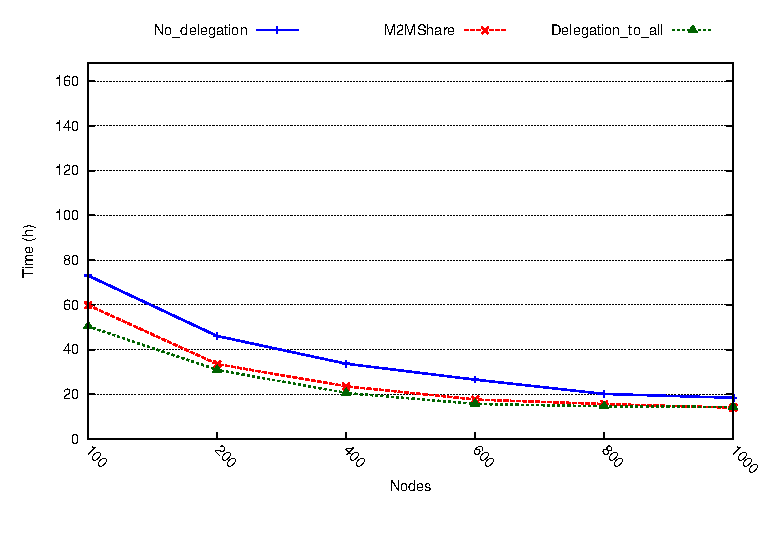
\includegraphics[scale=0.5]{grafici/tempiVF_Fp10.eps}
%\caption{Average found time with $Fp = 10\%$}
%\label{graficiTempiVF_Fp10}
%\end{minipage}
%\hspace{0.5cm}
%\begin{center}
%\begin{minipage}[b]{0.5\linewidth}
%\centering
%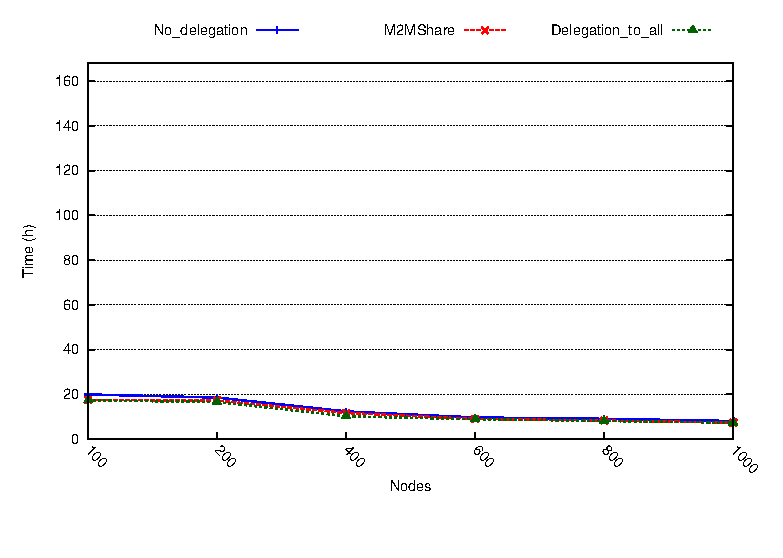
\includegraphics[scale=0.5]{grafici/tempiVF_Fp50.eps}
%\caption{Average found time with $Fp = 50\%$}
%\label{graficiTempiVF_Fp50}
%\end{minipage}
%\end{center}
%\end{figure}

\begin{figure}[htbp]
\centering%
\subfigure%
{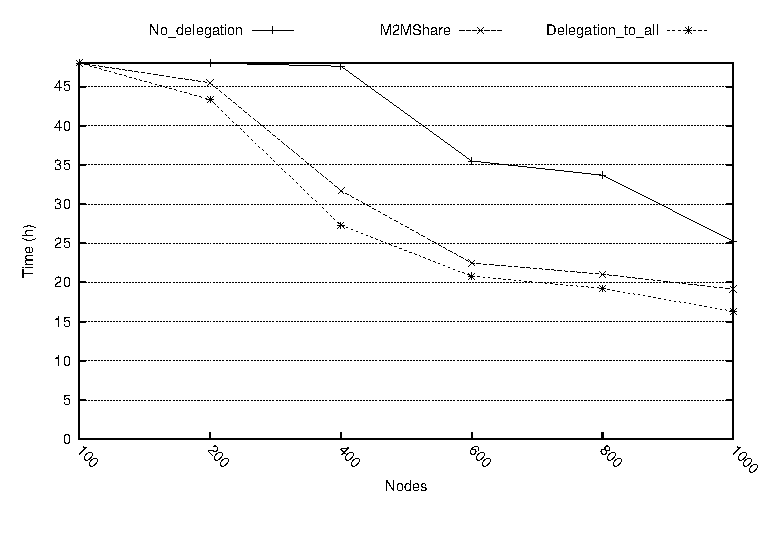
\includegraphics{grafici/tempiVF_Fp5.eps}}\qquad\qquad
\subfigure%
{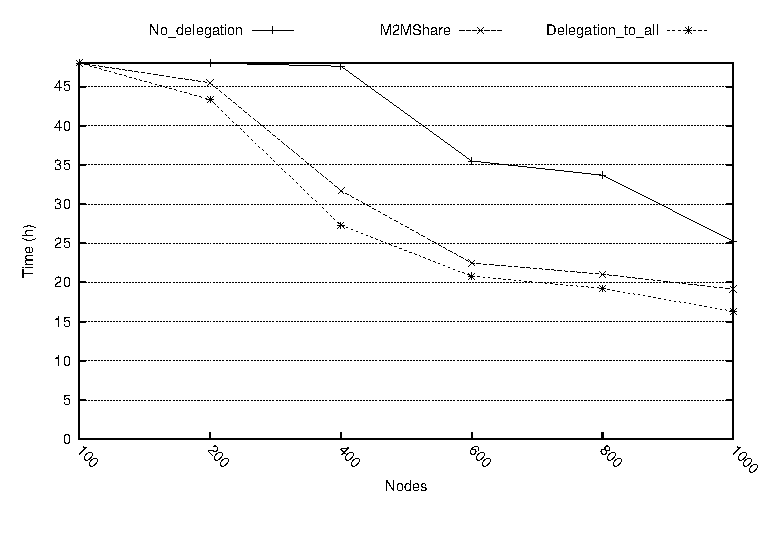
\includegraphics{grafici/tempiVF_Fp5_zoom.eps}}
\caption{Average found time with Fp $= 5\%$\label{graficiTempiVF_Fp5}}
\end{figure}

\begin{figure}[htbp]
\centering%
\subfigure%
{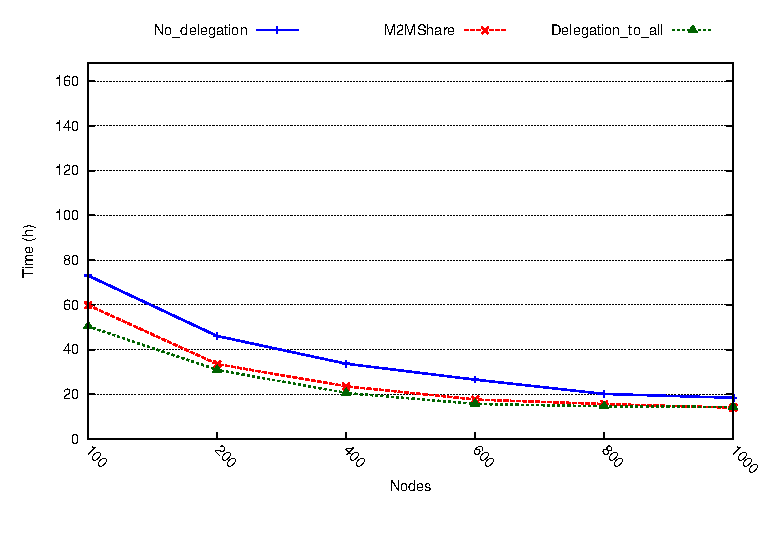
\includegraphics{grafici/tempiVF_Fp10.eps}}\qquad\qquad
\subfigure%
{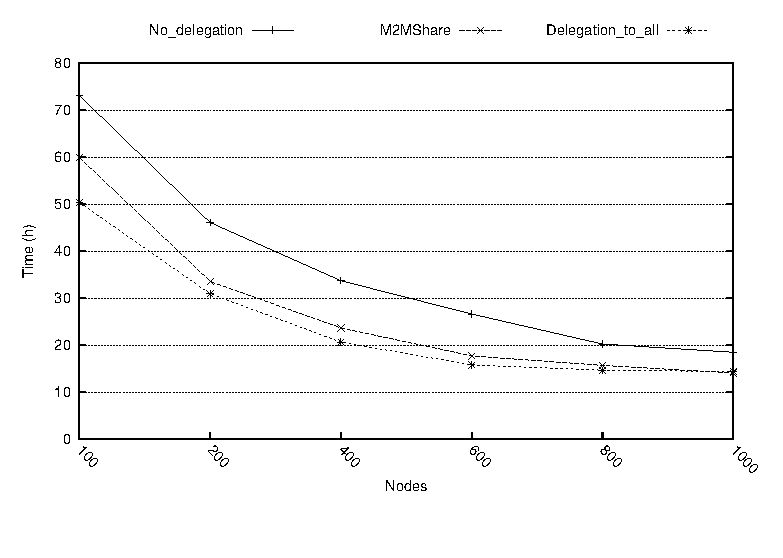
\includegraphics{grafici/tempiVF_Fp10_zoom.eps}}
\caption{Average found time with Fp $= 10\%$\label{graficiTempiVF_Fp10}}
\end{figure}

\begin{figure}[htbp]
\centering%
\subfigure%
{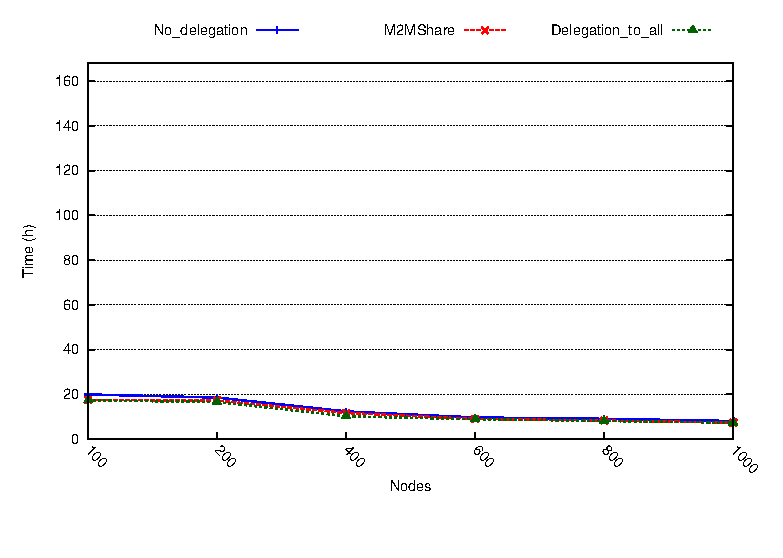
\includegraphics{grafici/tempiVF_Fp50.eps}}\qquad\qquad
\subfigure%
{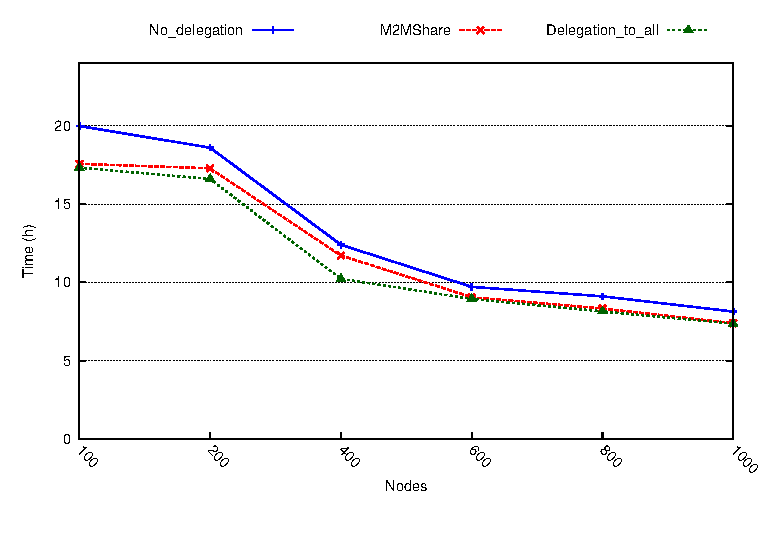
\includegraphics{grafici/tempiVF_Fp50_zoom.eps}}
\caption{Average found time with Fp $= 50\%$\label{graficiTempiVF_Fp50}}
\end{figure}



\newpage
\subsection{Data redundancy}
\label{analisiRidondanza}
\begin{table}[h]
\begin{center}
\begin{tabular}{|l|r|}
\hline
\bfseries Population & 1000 \\
\hline
\bfseries File size & 3.0 MB \\
\hline
\bfseries File popularity & 5\% \\
\hline
\bfseries File distribution & Uniformly distributed \\
\hline
\bfseries Delegation type & M2MShare, Delegation\_to\_all \\
\hline
\bfseries Delegation depth & 1 \\
\hline
\bfseries File Division Strategy & M2MShare \\
\hline
\bfseries Nr. of simulations & 40 x 2\\
\hline
\bfseries Simulated time & One week \\
\hline
\end{tabular}
\end{center}
\caption{Simulations settings for evaluation of data redundancy in the entire network\label{tab:settingsRedundancy}}
\end{table}

In analysis in Section \ref{analisiDelegationEfficiency}, especially in \figurename~ \ref{graficoDataDiverseDel}, we show that our system is the most efficient with respect to data transmissions. Although using delegations introduces an overhead in terms of bandwidth usage we control this side effects by delegating only to frequently encountered peers which are expected to be encountered again in the future. Another side effect caused by delegating tasks is the increasing of data redundancy in the whole network. For \textit{redundancy}, in this case, we mean storage space used in nodes involved in delegation system. 
\\ 

Of course redundancy in a network composed only by nodes which do not use delegation is always zero. For this reason, for this study we compare only the two systems which use task delegations and settings used for these simulations are shown in \tablename~\ref{tab:settingsRedundancy}. In \figurename~\ref{graficoRidondanzaData} we show how the average data redundancy changes during the progress of simulations. It is straightforward to notice the higher value introduced by delegating to all encountered peers whether M2MShare reduces the data redundancy quantity while still achieving the goal of acquiring the requested file. This is due to the number of contemporary active delegated tasks, shown in \figurename~\ref{graficoDelegheAttive}, which is higher in the system which delegates tasks to all encounter nodes. 
\\
The trend of this graph is related to the number of simultaneously active delegated tasks, shown in \figurename~\ref{graficoDelegheAttive}. Whenever a task is delegated, there is one more node looking for the searched file, and if it is found, the node will copy some file interval in its own data storage, and by so doing increasing the total data redundancy. On the other hand, when a delegated task expires, or a servant returns the output back to the requester node, temporary data downloaded for the task is deleted, freeing space in servant data storage and decreasing the total data redundancy.

\begin{figure}[htbp]
\begin{minipage}[b]{1\linewidth}
\centering
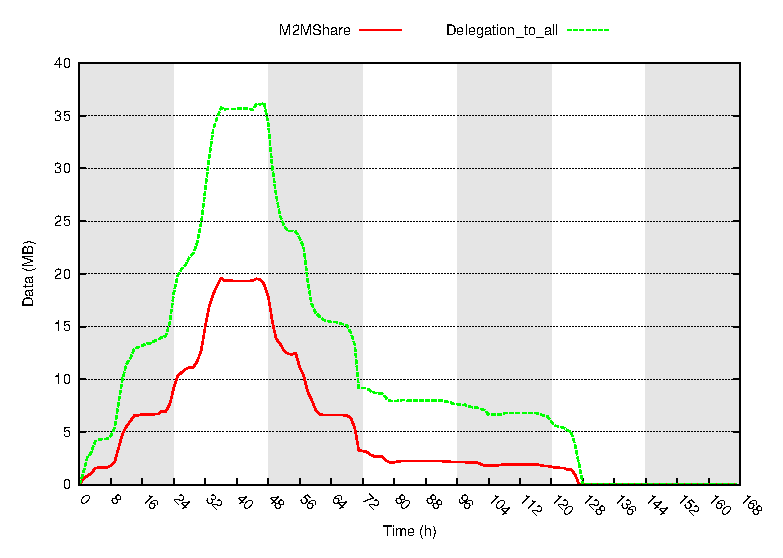
\includegraphics{grafici/ridondanza.eps}
\caption{Average data redundancy in the network}
\label{graficoRidondanzaData}
\end{minipage}
\hspace{0.5cm}
\begin{minipage}[b]{1\linewidth}
\centering
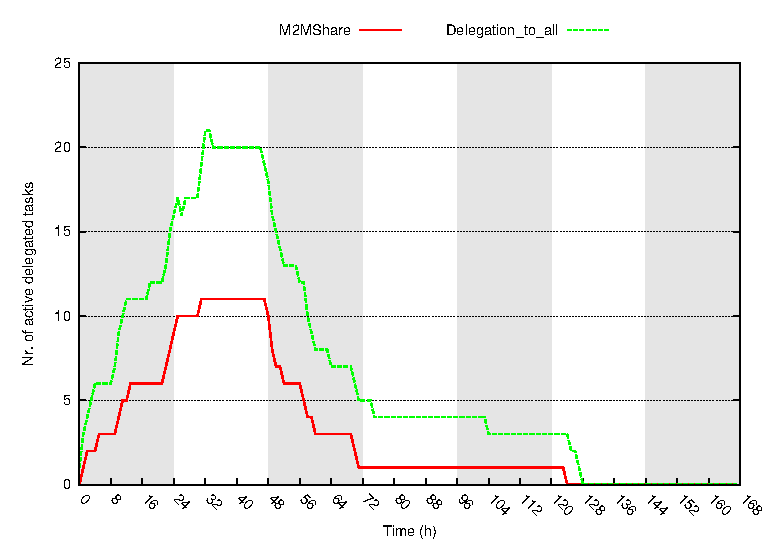
\includegraphics{grafici/delegheAttive.eps}
\caption{Average number of simultaneously active delegated tasks}
\label{graficoDelegheAttive}
\end{minipage}
\end{figure}


\newpage
\section{Multi-hop delegation efficiency}

\begin{table}[h]
\begin{center}
\begin{tabular}{|l|r|}
\hline
\bfseries Population & 1000 \\
\hline
\bfseries File size & 3.0 MB \\
\hline
\bfseries File popularity & 2,5\% \\
\hline
\bfseries File distribution & Distributed in a single district \\
\hline
\bfseries Delegation type & M2MShare\\
\hline
\bfseries Delegation depth & 1, 2, 3 \\
\hline
\bfseries Multi-hop delegation probability (MhDP) & 10\%, 25\%, 50\%, 75\%, 100\% \\
\hline
\bfseries File Division Strategy & M2MShare \\
\hline
\bfseries Nr. of simulations & 40 x 3 x 5\\
\hline
\bfseries Simulated time & One week \\
\hline
\end{tabular}
\end{center}
\caption{Simulations settings for evaluation of multi-hop delegation efficiency\label{tab:settingsMultiHop}}
\end{table}
In previous analysis we considered only delegation strategies using single-hop delegation, i.e. once a servant peer receives a task, delegated from another node, it will not delegate it again to a further-lever servant. 
\\

There are some situations in which single-hop delegations are not enough, due to other factors, like a low popularity of the searched file or its high distance from the searching peer. It is also possible that all the peers holding the searched file have different behaviours from those of the client and his direct servants. In these cases, we extended M2MShare by giving a peer the ability to delegate a pending task again. To avoid creating an excessively large number of delegations, we allow it to delegate again only after a trial period, i.e. one day, in which the servant tries to complete the task by itself. At the end of this period, if the task is still incomplete it is delegated again to a new set of upper-level servants.
\\

We simulate the behaviour of our protocol in a similar situation by tuning the distribution of the searched file at the beginning of the simulation: we distribute the initial 25 copies only between nodes in a map district on the other side of town from the searching node. As usual we repeated the simulations several times to obtain more accurate results, independently from the initial location of the searching node. In every simulation we then compare then the effectiveness of three different strategies:
\begin{itemize}
\item M2MShare with 1-hop delegations
\item M2MShare with up to 2-hop delegations
\item M2MShare with up to 3-hop delegations
\end{itemize}


An higher number of servant nodes involved in the delegation system results in a higher data redundancy added to the network. To limit the number of delegations used, we implement the multi-hop delegation system using different Multi-hop Delegation Probability (MhDP). This value indicates the probability that a node would re-delegate an incomplete task in a multi-hop system. As shown in \tablename~\ref{tab:settingsMultiHop}, we repeated our simulations with MHDP values of 10\%, 25\%, 50\%, 75\% and 100\%.
\\

In \figurename~\ref{fig:tempiVF_MultiHop} it is possible to see the average found time employed  by the three strategies to return the searched file to the requester node. M2MShare with 1-hop delegations can achieve some success, but it is not comparable with results of M2MShare versions employing multi-hop delegations. The two systems using multi-hop delegations find the required file in less time in each simulation run at the expense of higher overhead in terms of number of servant peers involved, as we will see in Section \ref{analisiRidondanzaMultiHop}.

\begin{figure}[htpb]
  \begin{center}
    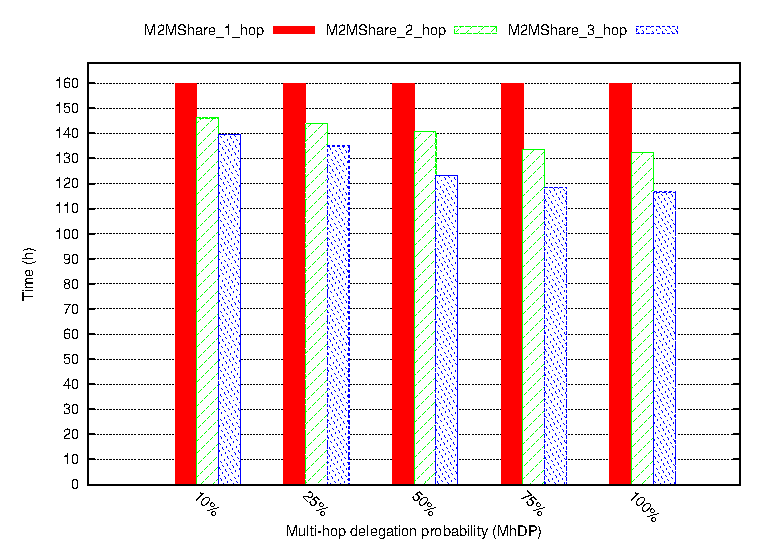
\includegraphics{grafici/tempiVF_MultiHop.eps}
    \caption{Average found time employed by M2MShare with different multi-hop versions in finding the required data file.}
    \label{fig:tempiVF_MultiHop}
  \end{center}
\end{figure}

%\begin{figure}[ht]
%\begin{minipage}[b]{1\linewidth}
%\centering
%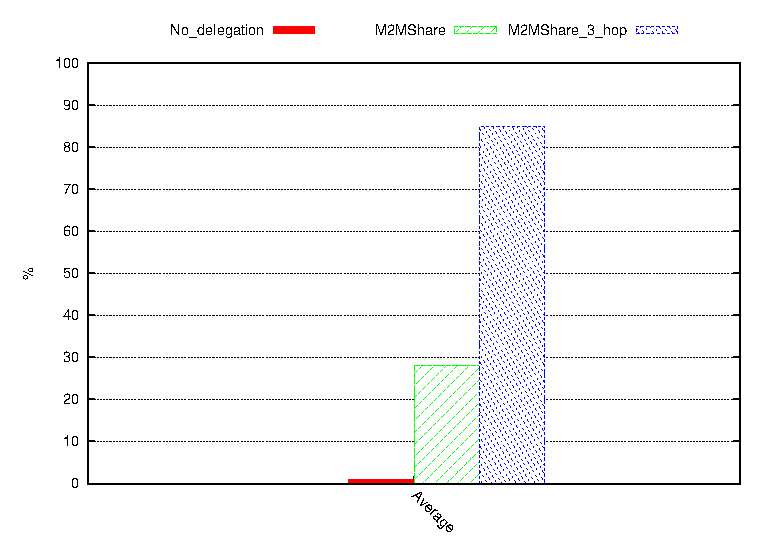
\includegraphics[scale=0.5]{grafici/percCompletaMultiHop.eps}
%\caption{Percentage of successfully completed simulations.}
%\label{graficoPercCompletedMultiHop}
%\end{minipage}
%\end{figure}

\newpage
\subsection{Map coverage}
It is straightforward that re-delegating a unaccomplished task extends the total explored area. A single node can explore only a small area, covered only by its own connectivity range. With M2MShare 1-hop version there is an increase of the explored area, due to delegations to some servants with different movement behaviour than the requester, but limited to 1-hop delegation. With multi-hop delegation there is a maximum extension of the coverage area. In this analysis we evaluate the average explored area using different values of delegation depth and MhDP.
\\

First of all we create a control set to evaluate the maximum area that can be explored by nodes during the simulations. To do so we execute 40 simulations with nodes involved in their daily activities, but with no files distributed and no file request in one node. Settings for these simulations are shown in \tablename~\ref{tab:settingsControlSet}. We evaluate the average area explored by all 1000 nodes in one-week simulations. The related map is shown in  \figurename~\ref{fig:mapCoverage_controlSet}. We adopt this value to the maximum area that can be explored (100\%) and we repeate a set of simulations using values in \tablename~\ref{tab:settingsMultiHop}: we compare M2MShare with 1-hop, 2-hop and 3-hop delegations and using different Multi-hop Delegation Probability (MhDP). The average area explored using different MhDP values is shown in \figurename~\ref{fig:mapCoverage_MultiHop}.
\\
As it is possible to see, M2MShare expands the explored area of a single due to delegations to some servants with different movement behaviour than the requester, but limited to 1-hop delegation. The maximum area extension is when using up to 3-hop delegations in which almost the entire city is covered by searching nodes.
\\

For each MhDP value we show the differences in explored area using 1-hop, 2-hop or 3-hop delegations. In \figurename~\ref{fig:mappaMultiHop_10} we show the tree maps related to the average explored area using the three versions of M2MShare with MhDP~$= 10\%$. Raising the MhDP value to 25\% (\figurename~\ref{fig:mappaMultiHop_25}) it is possible to see an increment of the explored area using multi-hop delegations. This increment is less visible increasing the MhDP again to 50\% (\figurename~\ref{fig:mappaMultiHop_50}), 75\% (\figurename~\ref{fig:mappaMultiHop_75}) or 100\% (\figurename~\ref{fig:mappaMultiHop_100}).   

\begin{table}[htpb]
\begin{center}
\begin{tabular}[width=4cm]{|l|r|}
\hline
\bfseries Population & 1000 \\
\hline
\bfseries File distribution & No file distributed \\
\hline
\bfseries Delegation type & No\_Delegation \\
\hline
\bfseries Nr. of simulations & 40\\
\hline
\bfseries Simulated time & One week \\
\hline
\end{tabular}
\end{center}
\caption{Simulations settings for map coverage control set\label{tab:settingsControlSet}}
\end{table}

\begin{figure}[htpb]
  \begin{center}
    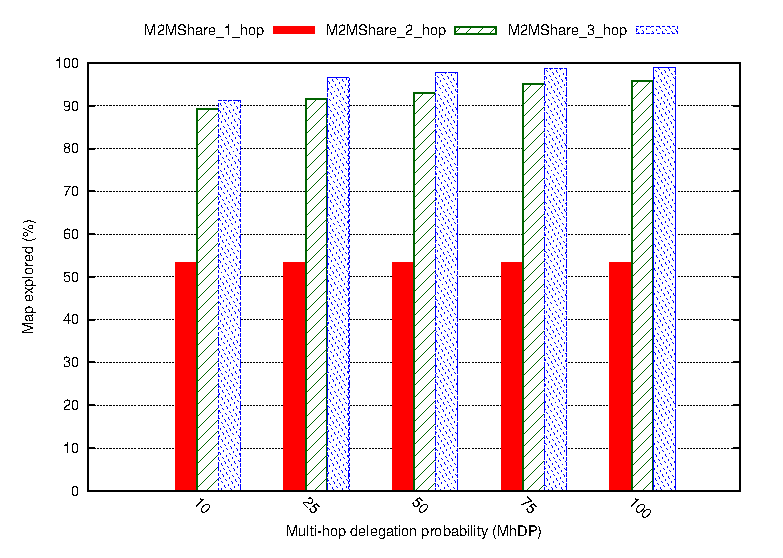
\includegraphics{grafici/mapCovered_MultiHop.eps}
    \caption{Average percentage of explored area employing M2MShare with different multi-hop versions.}
    \label{fig:mapCoverage_MultiHop}
  \end{center}
\end{figure}

\begin{figure}[htpb]
  \begin{center}
    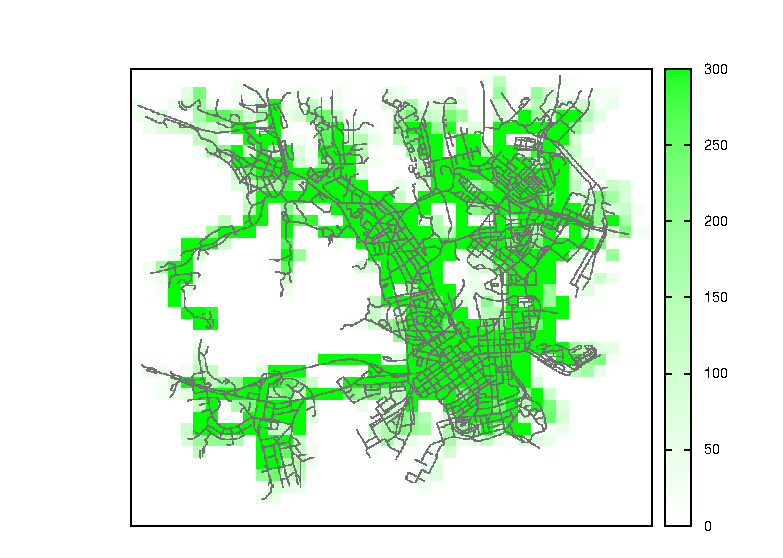
\includegraphics[scale=0.85]{grafici/mappe/controlSet.eps}
    \caption{Maximum explored area by nodes in one-week simulations.}
    \label{fig:mapCoverage_controlSet}
  \end{center}
\end{figure}


\begin{figure}[htbp]
\centering%
\vspace{-30pt}%
\subfigure[Explored area with 1-hop delegations]%
{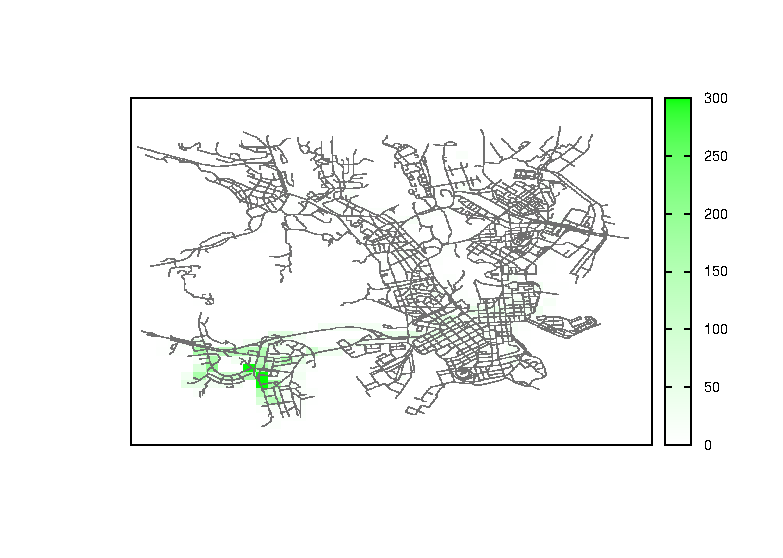
\includegraphics[scale=0.85]{grafici/mappe/M2MShare_1_hop_10perc.eps}}\qquad
\vspace{-10pt}%
\subfigure[Explored area with 2-hop delegations]%
{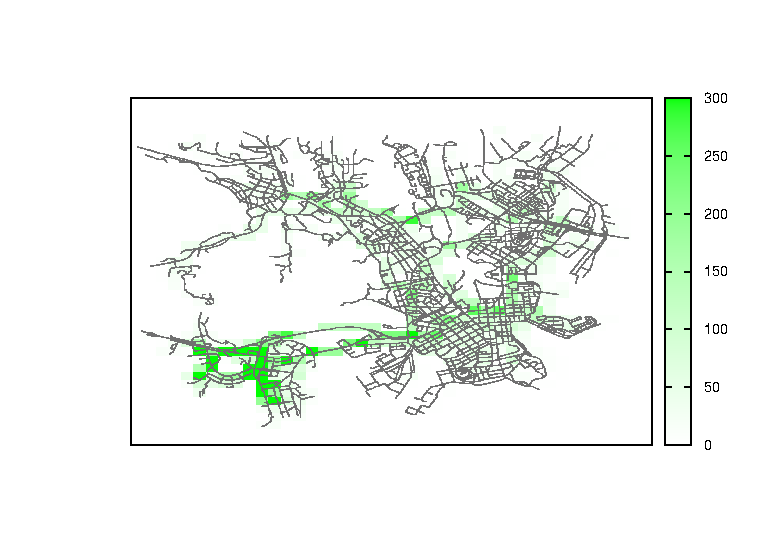
\includegraphics[scale=0.85]{grafici/mappe/M2MShare_2_hop_10perc.eps}}\qquad
\vspace{-10pt}%
\subfigure[Explored area with 3-hop delegations]%
{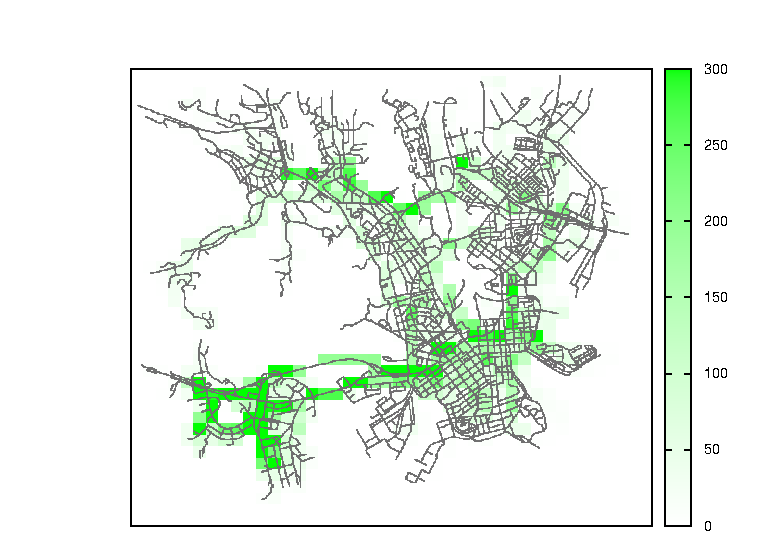
\includegraphics[scale=0.85]{grafici/mappe/M2MShare_3_hop_10perc.eps}}
\caption{Average explored area with MhDP $= 10\%$\label{fig:mappaMultiHop_10}}
\end{figure}

\begin{figure}[htbp]
\centering%
\vspace{-30pt}%
\subfigure[Explored area with 1-hop delegations]%
{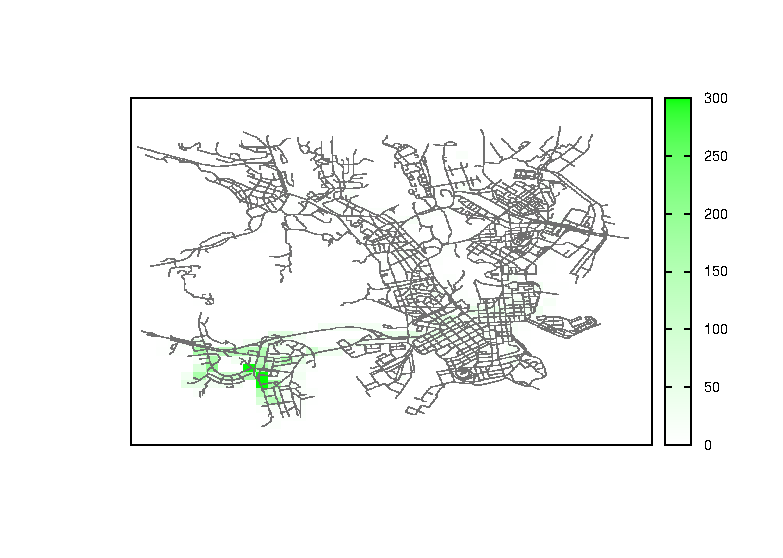
\includegraphics[scale=0.85]{grafici/mappe/M2MShare_1_hop_25perc.eps}}\qquad
\vspace{-10pt}%
\subfigure[Explored area with 2-hop delegations]%
{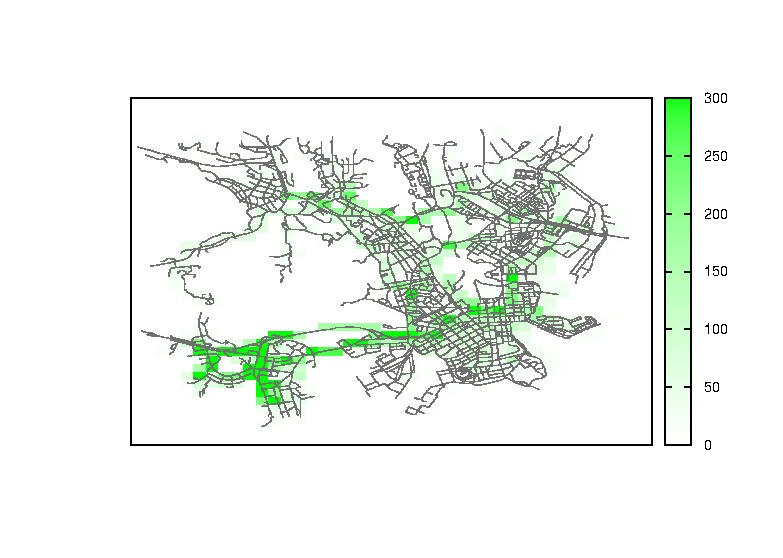
\includegraphics[scale=0.85]{grafici/mappe/M2MShare_2_hop_25perc.eps}}\qquad
\vspace{-10pt}%
\subfigure[Explored area with 3-hop delegations]%
{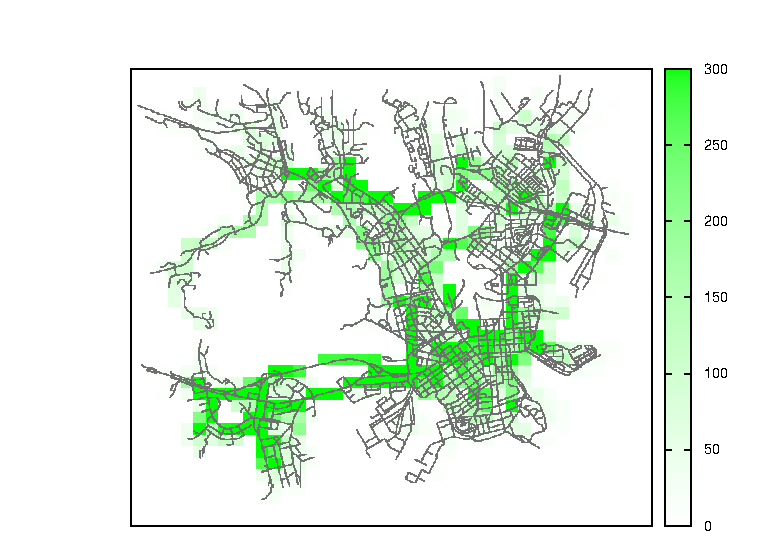
\includegraphics[scale=0.85]{grafici/mappe/M2MShare_3_hop_25perc.eps}}
\caption{Average explored area with MhDP $= 25\%$\label{fig:mappaMultiHop_25}}
\end{figure}

\begin{figure}[htbp]
\centering%
\vspace{-30pt}%
\subfigure[Explored area with 1-hop delegations]%
{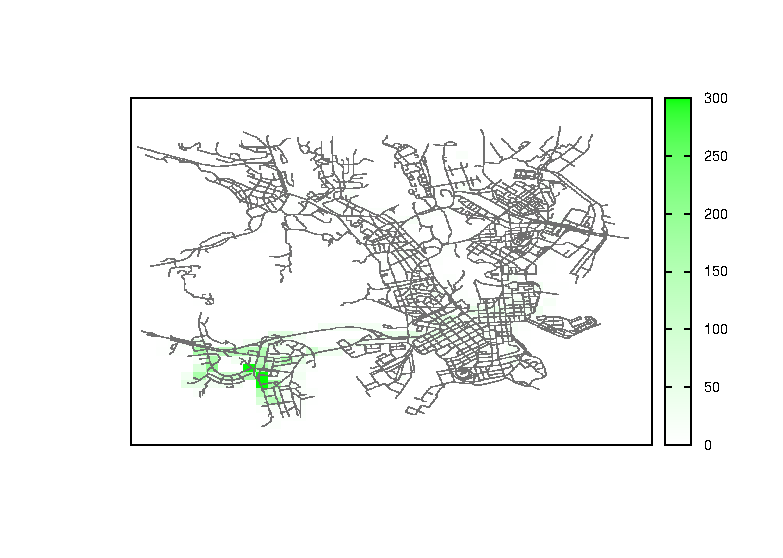
\includegraphics[scale=0.85]{grafici/mappe/M2MShare_1_hop_50perc.eps}}\qquad
\vspace{-10pt}%
\subfigure[Explored area with 2-hop delegations]%
{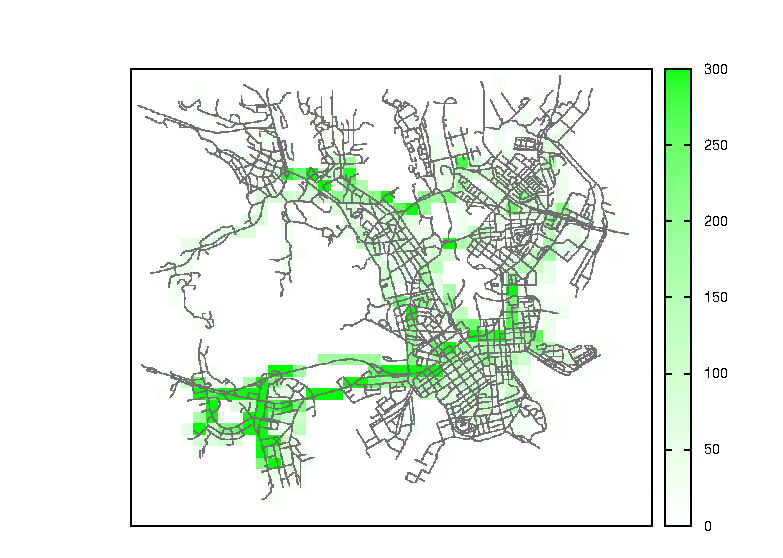
\includegraphics[scale=0.85]{grafici/mappe/M2MShare_2_hop_50perc.eps}}\qquad
\vspace{-10pt}%
\subfigure[Explored area with 3-hop delegations]%
{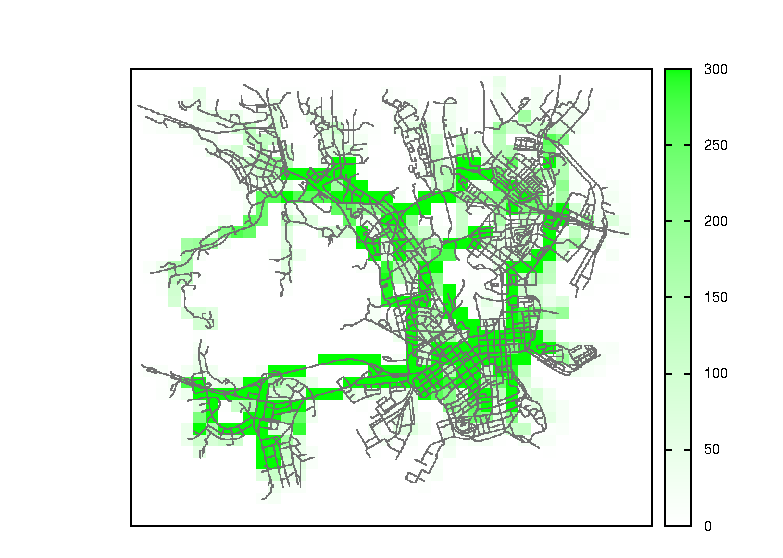
\includegraphics[scale=0.85]{grafici/mappe/M2MShare_3_hop_50perc.eps}}
\caption{Average explored area with MhDP $= 50\%$\label{fig:mappaMultiHop_50}}
\end{figure}

\begin{figure}[htbp]
\centering%
\vspace{-30pt}%
\subfigure[Explored area with 1-hop delegations]%
{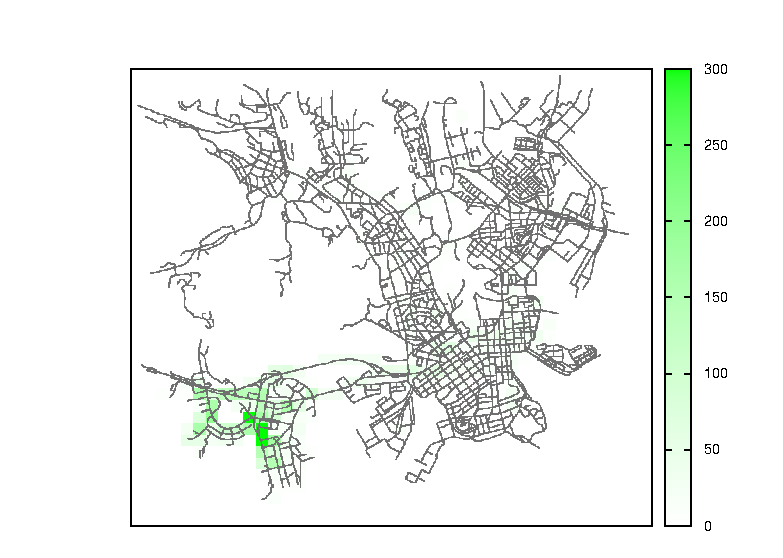
\includegraphics[scale=0.85]{grafici/mappe/M2MShare_1_hop_75perc.eps}}\qquad
\vspace{-10pt}%
\subfigure[Explored area with 2-hop delegations]%
{\includegraphics[scale=0.85]{grafici/mappe/M2MShare_2_hop_75perc.eps}}\qquad
\vspace{-10pt}%
\subfigure[Explored area with 3-hop delegations]%
{\includegraphics[scale=0.85]{grafici/mappe/M2MShare_3_hop_75perc.eps}}
\caption{Average explored area with MhDP $= 75\%$\label{fig:mappaMultiHop_75}}
\end{figure}

\begin{figure}[htbp]
\centering%
\vspace{-30pt}%
\subfigure[Explored area with 1-hop delegations]%
{\includegraphics[scale=0.85]{grafici/mappe/M2MShare_1_hop_100perc.eps}}\qquad
\vspace{-10pt}%
\subfigure[Explored area with 2-hop delegations]%
{\includegraphics[scale=0.85]{grafici/mappe/M2MShare_2_hop_100perc.eps}}\qquad
\vspace{-10pt}%
\subfigure[Explored area with 3-hop delegations]%
{\includegraphics[scale=0.85]{grafici/mappe/M2MShare_3_hop_100perc.eps}}
\caption{Average explored area with MhDP $= 100\%$\label{fig:mappaMultiHop_100}}
\end{figure}




%As it is possible to see in \figurename~\ref{mappa0Hop}, the strategy which does not use delegations explores only a small area, covered only by its own connectivity range. With M2MShare (in \figurename~\ref{mappa1Hop}) there is an increase of the explored area, due to delegations to some servants with different movement behaviour than the requester, but limited to 1-hop delegation. The maximum area extension is when using up to 3-hop delegations in which, as we can see in \figurename~\ref{mappa3Hop}, almost all the city is covered by searching nodes.

%\begin{figure}[htpb]
%  \begin{center}
%    \includegraphics[scale=0.35]{figure/mappa_0_hop.png}
%    \caption{Explored area without use of delegations}
%    \label{mappa0Hop}
%  \end{center}
%\end{figure}
%
%\begin{figure}[htpb]
%  \begin{center}
%    \includegraphics[scale=0.35]{figure/mappa_1_hop.png}
%    \caption{Explored area using M2MShare and 1-hop delegations}
%    \label{mappa1Hop}
%  \end{center}
%\end{figure}
%
%\begin{figure}[htpb]
%  \begin{center}
%    \includegraphics[scale=0.35]{figure/mappa_3_hop.png}
%    \caption{Explored area using M2MShare and up to 3-hop delegations}
%    \label{mappa3Hop}
%  \end{center}
%\end{figure}

\newpage
\subsection{Data redundancy}
\label{analisiRidondanzaMultiHop}
In analysis in Section \ref{analisiRidondanza} we show the redundancy added in the network by using delegation and we show how our system outperforms the other trivial system which uses delegation to all encountered peers. In current section we show the impact of using multi-hop delegation respect to added redundancy in the network. For these simulations we use the settings shown in \tablename~\ref{tab:settingsMultiHop}. We compared three versions of M2MShare with different maximum number of delegation hops. We also changed the probability that a servant peer would delegate again a received pending task.
\\

In \figurename~\ref{fig:ridondanzaMultiHop_10}, \ref{fig:ridondanzaMultiHop_25}, \ref{fig:ridondanzaMultiHop_50}, \ref{fig:ridondanzaMultiHop_75}, \ref{fig:ridondanzaMultiHop_100} we can see the difference in number of delegation used and data redundancy added by the three versions of M2MShare. Both of them use the same number of delegations for the first day, then the 2-hop and the 3-hop versions start to delegate again the incomplete task. The next difference can be seen after another day, when nodes adopting 3-hop delegations again delegate the unaccomplished task. It is straightforward to notice the increment of servant nodes using 3-hop delegations versus 2-hop or 1-hop systems.
\\

A higher number of servant nodes involved in the delegation system results in a higher data redundancy added to the network. To limit the number of delegations used and related data redundancy added, we implement the multi-hop delegation system using different Multi-hop Delegation Probability (MhDP). This value indicates the probability that a node would delegate again an incomplete task in a multi-hop system. We repeated our simulations with MhDP values of 10\% (\figurename~\ref{fig:ridondanzaMultiHop_10}), 25\% (\figurename~\ref{fig:ridondanzaMultiHop_25}), 50\% (\figurename~\ref{fig:ridondanzaMultiHop_50}), 75\% (\figurename~\ref{fig:ridondanzaMultiHop_75}) and 100\% (\figurename~\ref{fig:ridondanzaMultiHop_100}). With a small MhDP value a small number of delegations are used, reducing the overall data redundancy. Raising MhDP value, more delegations are used, increasing the data redundancy introduced into the network. With MhDP \= 100\% a servant peer delegates a unaccomplished task to every encountered node which exceeds Frequency Threshold value, after the one-day trial period. With a such high MhDP value we can see that over 70\% of nodes in the simulation are involved in delegations system.


\begin{figure}[htbp]
\centering%
\subfigure[Data redundancy in the network]%
{\includegraphics{grafici/ridondanza_multiHop_10perc.eps}}\qquad\qquad
\subfigure[Number of simultaneously active delegated tasks]%
{\includegraphics{grafici/delegheAttive_multiHop_10perc.eps}}
\caption{Average data redundancy and number of active delegated tasks with MhDP $= 10\%$\label{fig:ridondanzaMultiHop_10}}
\end{figure}

\begin{figure}[htbp]
\centering%
\subfigure[Data redundancy in the network]%
{\includegraphics{grafici/ridondanza_multiHop_25perc.eps}}\qquad\qquad
\subfigure[Number of simultaneously active delegated tasks]%
{\includegraphics{grafici/delegheAttive_multiHop_25perc.eps}}
\caption{Average data redundancy and number of active delegated tasks with MhDP $= 25\%$\label{fig:ridondanzaMultiHop_25}}
\end{figure}

\begin{figure}[htbp]
\centering%
\subfigure[Data redundancy in the network]%
{\includegraphics{grafici/ridondanza_multiHop_50perc.eps}}\qquad\qquad
\subfigure[Number of simultaneously active delegated tasks]%
{\includegraphics{grafici/delegheAttive_multiHop_50perc.eps}}
\caption{Average data redundancy and number of active delegated tasks with MhDP $= 50\%$\label{fig:ridondanzaMultiHop_50}}
\end{figure}

\begin{figure}[htbp]
\centering%
\subfigure[Data redundancy in the network]%
{\includegraphics{grafici/ridondanza_multiHop_75perc.eps}}\qquad\qquad
\subfigure[Number of simultaneously active delegated tasks]%
{\includegraphics{grafici/delegheAttive_multiHop_75perc.eps}}
\caption{Average data redundancy and number of active delegated tasks with MhDP $= 75\%$\label{fig:ridondanzaMultiHop_75}}
\end{figure}

\begin{figure}[htbp]
\centering%
\subfigure[Data redundancy in the network]%
{\includegraphics{grafici/ridondanza_multiHop_100perc.eps}}\qquad\qquad
\subfigure[Number of simultaneously active delegated tasks]%
{\includegraphics{grafici/delegheAttive_multiHop_100perc.eps}}
\caption{Average data redundancy and number of active delegated tasks with MhDP $= 100\%$\label{fig:ridondanzaMultiHop_100}}
\end{figure}
%
%Of course redundancy in a network composed only by nodes which do not use delegation is always zero. For this reason, for this study we compared only the two systems which use task delegations and settings used for these simulations are shown in \tablename~\ref{tab:settingsRedundancy}. In \figurename~\ref{graficoRidondanzaData} we show how change the average data redundancy during the progress of simulations. It is straightforward to notice the higher value introduced by delegating to all encountered peers whether M2MShare reduces the data redundancy quantity while still achieving the goal of acquiring the requested file. This is due to the number of contemporary active delegated tasks, shown in \figurename~\ref{graficoDelegheAttive}, which is higher in the system which delegates task to all encounter nodes. 
%\\
%The trend of this graph is related to the number of simultaneously active delegated tasks, shown in \figurename~\ref{graficoDelegheAttive}. Whenever a task is delegated, there is one more node looking for the searched file, and if it is found, the node will copy some file interval in its own data storage, doing so increase the total data redundancy. On the other hand, when a delegated task expires, or a servant returns the output to the requester node, temporary data downloaded for the task is deleted, freeing space in servant's data storage and doing decrease the total data redundancy.

\newpage 
\section{File Division Strategy efficiency}
\begin{table}[h]
\begin{center}
\begin{tabular}{|l|r|}
\hline
\bfseries Population & 1000 \\
\hline
\bfseries File size & 3.0 MB, 10.0 MB, 25.0 MB \\
\hline
\bfseries File popularity & 5\% \\
\hline
\bfseries File distribution & Uniformly distributed \\
\hline
\bfseries Delegation type & M2MShare \\
\hline
\bfseries Delegation depth & 1 \\
\hline
\bfseries File Division Strategy & M2MShare, iM , rM \\
\hline
\bfseries Nr. of simulations & 40 x 3 x 3\\
\hline
\bfseries Simulated time & One week \\
\hline
\end{tabular}
\end{center}
\caption{Simulations settings for evaluation of file division strategy efficiency\label{tab:settingsFDS}}
\end{table}
In previous analysis we evaluate the efficiency of M2MShare delegation technique, but in the protocol the delegation system is not the only new innovation described. M2MShare provides a new file division strategy, described in Section \ref{descrFileDivisionStrategy}, where a file can be downloaded in pieces and a piece size varies. File division strategy might add redundancy during data transfer as it can happen that overlapping data intervals are simultaneously downloaded by different servants. However, the fact that each servant is asked to download the file starting from different points allows reconstructing the whole file even if both downloaded only part of it. \\
As shown in \tablename~\ref{tab:settingsFDS} we compare our file division strategy with two other division strategies:
\begin{itemize}
\item iM: a strategy which requests at each file server the entire file, always starting from its first byte;
\item rM: a strategy that randomly chooses the initial download point in the file request.
\end{itemize}

We considered the average, min and max transferred data amount employed in each file division strategy. We repeated the simulations 40 times, changing random seeds, for every file division strategy in order to achieve more accurate results and we did this using three different sizes for the searched file. 
\\
In earlier studies some test were done to evaluate the efficiency of M2MShare file division strategy, but task delegation was not considered because simulated scenarios did not take into consideration disconnections due to mobility or interferences that happen in real world
communication. That has only been possible with the current implementation of the protocol, in a network simulation environment which can simulate movement of nodes emulating people using M2MShare.
In \figurename~\ref{graficoDataFDS_3MB}, \figurename~\ref{graficoDataFDS_10MB} and \figurename~\ref{graficoDataFDS_25MB} we can see that our division strategy has the least redundancy during data transfer, especially considering big-sized files.

\begin{figure}[htbp]
\centering%
\subfigure%
{\includegraphics{grafici/dataDFS_3MB.eps}}\qquad\qquad
\subfigure%
{\includegraphics{grafici/dataDFS_3MB_zoom.eps}}
\caption{Average, min, max transferred data amount using different file division strategies and 3.0 MB file size.\label{graficoDataFDS_3MB}}
\end{figure}

\begin{figure}[htbp]
\centering%
\subfigure%
{\includegraphics{grafici/dataDFS_10MB.eps}}\qquad\qquad
\subfigure%
{\includegraphics{grafici/dataDFS_10MB_zoom.eps}}
\caption{Average, min, max transferred data amount using different file division strategies and 10.0 MB file size.\label{graficoDataFDS_10MB}}
\end{figure}

\begin{figure}[htbp]
\centering%
\subfigure%
{\includegraphics{grafici/dataDFS_25MB.eps}}\qquad\qquad
\subfigure%
{\includegraphics{grafici/dataDFS_25MB_zoom.eps}}
\caption{Average, min, max transferred data amount using different file division strategies and 25.0 MB file size.\label{graficoDataFDS_25MB}}
\end{figure}

%\begin{figure}[ht]
%\begin{minipage}[b]{0.5\linewidth}
%\centering
%\includegraphics[scale=0.5]{grafici/dataDFS_3MB.eps}
%\caption{Average, min, max transferred data amount using different file division strategies and 3.0 MB file size.}
%\label{graficoDataFDS_3MB}
%\end{minipage}
%\hspace{0.5cm}
%\begin{minipage}[b]{0.5\linewidth}
%\centering
%\includegraphics[scale=0.5]{grafici/dataDFS_10MB.eps}
%\caption{Average, min, max transferred data amount using different file division strategies and 10.0 MB file size.}
%\label{graficoDataFDS_10MB}
%\end{minipage}
%\hspace{0.5cm}
%\begin{center}
%\begin{minipage}[b]{0.5\linewidth}
%\centering
%\includegraphics[scale=0.5]{grafici/dataDFS_25MB.eps}
%\caption{Average, min, max transferred data amount using different file division strategies and 25.0 MB file size.}
%\label{graficoDataFDS_25MB}
%\end{minipage}
%\end{center}
%\end{figure}


%\label{analisiLabel}
 
% ---------------------------------------------------------------------------
%: ----------------------- end of thesis sub-document ------------------------
% ---------------------------------------------------------------------------


% this file is called up by thesis.tex
% content in this file will be fed into the main document

%: ----------------------- name of chapter  -------------------------
\chapter{Conclusions}\label{conclusioni} % top level followed by section, subsection




%: ----------------------- contents from here ------------------------
%In this thesis, we evaluated the performance of M2MShare, a protocol which implements DTN techniques in mobile phones world, in order to enable a peer-to-peer file sharing system between peers in the network making leverage on their mobility and opportunistic contacts among them. To do so we implemented the protocol in the Oppostunistic Network Environment (ONE) simulator. This simulator is able to emulate human movements adopting several movement models in a map-based environment and allowing us to evaluate M2MShare behaviour in a realistic city-scale scenario.
In this thesis, we evaluated the performance of M2MShare, a DTN solution for mobile phones that leverages on nodes' mobility and opportunistic contacts to enable proximity based file sharing. To this aim, we have integrated M2MShare in the Opportunistic Network Environment (ONE) simulator and tested its performance with realistic movement models in a map-based environment. This complex city-scale testbed includes a multitude of nodes representing real users engaged in their daily activities and movements, and allowed us to demonstrate the efficacy of M2MShare. 
\\

We evaluated M2MShare employing one-hop delegations against two other systems using different strategies:
\begin{itemize}
\item \textit{No\_delegation:} a system which does not employ delegations and file exchange is initiated only when a peer holding the requested data file is found in reach area of file requester.
\item \textit{Delegation\_to\_all:} a system employing delegations but instead employs the trivial technique where missing tasks are delegated to each encountered peer.
\end{itemize}
Our analysis proved that the use of delegations is more efficient than the strategy which does not employ them, due to the number of servant peers involved in the file-search activity. This number is limited using as heuristic the history of met nodes and delegating tasks only to frequently encountered peers. We proved that this strategy allows M2MShare to be more efficient than the strategy in which tasks are indiscriminately delegated to all met peers, with respect to the number of peers involved and to the redundancy introduced in the entire network.
\\

We improved M2MShare by adding support for multi-hop delegations and we proved how this increases the search area for a file, compared to the single-hop delegations strategy introduced by M2MShare.
\\

We compared M2MShare file division strategy with two other division strategies:
\begin{itemize}
\item iM: a strategy which requests at each file server the entire file, always starting from its first byte;
\item rM: a strategy that randomly chooses the initial download point in the file request.
\end{itemize}
and we proved that our file division strategy has the least redundancy during data transfer, especially considering big-sized files.
\\

Some of the previous results will be presented with a paper we wrote at Wireless Days Conference 2011 \footnote{Wireless Days 2011 \href{http://www.wireless-days.org/}{http://www.wireless-days.org/}} in Niagara Falls, Ontario, Canada. The full text of the paper is included in Appendix \ref{appendice-paper}.
Summarizing, our contributions are the following:
\begin{itemize}
\item implementing M2MShare and evaluating its behaviour using a simulator (the ONE simulator) able to emulate nodes movement in a realistic urban scenario;
\item evaluating the efficiency of the new paradigm created by M2MShare of use P2P solutions that matches file sharing with mobile users, allowing them to exchange files with each other;
\item evaluating the efficiency of using task delegations to dynamically establish forward routes along the destination path in the network;
\item evaluating the efficiency of the new file division strategy introduced with M2MShare; 
\item enhancing M2MShare adding support to multi-hop delegations in order to further increase the search area for a single node to other disconnected overlay networks;
\item enhancing the ONE simulator adding some new features to it and then making them available to the simulator users community\footnote{The ONE simulator user contributions \href{http://www.netlab.tkk.fi/tutkimus/dtn/theone/\#contrib}{http://www.netlab.tkk.fi/tutkimus/dtn/theone/\#contrib}}.
\end{itemize}

\pagebreak
\section{Future Work}
There are other analysis that could be done to evaluate M2MShare efficiency, with respect to several factors. Some of them might be:
%Some potential future developments to further improve and extend the functionalities provided by the software might be:
\begin{itemize}
\item Wider scenario: we emulated M2MShare behaviour and evaluated its efficiency in a city-scale scenario, adopting the Working Day Movement Model to emulate users daily activities. An interesting future work could be to evaluate M2MShare performance in a wider-scale environment, say a scenario composed by multiple cities and emulating commuters moving from one city to the other during their daily activities.
\item Power consumption analysis: one characteristic of mobile devices is the limited power. One future analysis could be to evaluate the impact of delegations in terms of energy consumption. Several models for  energy consumption analysis for Bluetooth are available and could be adapted and implemented in the ONE simulator.
\item Search phase emulation: we emulated only the second part of the protocol, the one in which a node looks for a specific file and asks to other peers for it, using delegations. A possible future analysis would be to evaluate the efficiency of the Search Module of M2MShare in indexing and returning results for a user query, using delegations even for this activity.
\end{itemize}

\newpage
\section{Acknowledgements}
First of all, I have to thank my parents, Ganni and Gabriela, for the support they provided me through my entire life, for all their love and encouragement and for believe in me in every circumstance.\\

I must express my gratitude towards my advisor, professor Claudio Enrico Palazzi, for his supervision, guidance and advices in writing this thesis. \\

My thanks to my co-advisor, Armir Bujari, for his precious help and willingness throughout the work which lead to the realization of this thesis.\\

Special thanks to Silvia, for her persistent confidence in me, for motivating me and for always pushing me to do my best.\\

Thanks to my friend Yuri, who helped me during all these years we lived together as roommates.\\

My thanks to Alberto, Luca and everyone that worked and studied with me, friends before colleagues.\\

The support and encouragement of many other people has been indispensable during the last years, so I would show my gratitude to my friends, to everyone who has given me something, to everyone that has been with me, and to everyone I have not mentioned here.\\

\begin{flushright}
\textit{Daniele}
\end{flushright}

 
% ---------------------------------------------------------------------------
%: ----------------------- end of thesis sub-document ------------------------
% ---------------------------------------------------------------------------




\cleardoublepage 	 %va a pagina nuova iniziando dalla pagina di destra

%%%%%%%%%%%%%%%%%%%%%%%%%%%%%%%%%%%%%%%%%%%%%%%%%%%%%%%

%%%%%%%%%Facoltativi%%%%%%%%%%%%%%%%%%%%%%%%%%%%%%%%

%%%%%%%%%%%%%%%%%%CONCLUSIONI%%%%%%%%%%%%%%%%%%%%%%%%%%

%\rhead[\fancyplain{}{\bfseries                                              %imposta l'intestazione di pagina destra
%CONCLUSIONI}]{\fancyplain{}{\bfseries\thepage}}
%\lhead[\fancyplain{}{\bfseries\thepage}]{\fancyplain{}{\bfseries            %imposta l'intestazione di pagina sinistra
%CONCLUSIONI}}
%\addcontentsline{toc}{chapter}{Conclusioni}                                 %aggiunge la voce Conclusioni nell'indice
%\input{Conclusioni}                                                         %preleva il file in cui ci sono le conclusioni
%\cleardoublepage

%%%%%%%%%%%%%%%%%%%%%%%%%%%%%%%%%%%%%%%%%%%%%%%%%%%%%%%


%%%%%%%%%%%%%%%%%%%%APPENDICE%%%%%%%%%%%%%%%%%%%%%%%%%%%%%5

%\rhead[\fancyplain{}{\bfseries                                              %imposta l'intestazione di pagina destra
%APPENDICE}]{\fancyplain{}{\bfseries\thepage}}                               %imposta l'intestazione di pagina
%\lhead[\fancyplain{}{\bfseries\thepage}]{\fancyplain{}{\bfseries            %imposta l'intestazione di pagina (si pu� cambiare la scritta appendice con il suo nome in modo da far apparire nella intestazione della pagina sinistra il nome dell'appendice)
%APPENDICE}} \addcontentsline{toc}{chapter}{Appendice: Data Sheet}
%\input{Appendice}
%\cleardoublepage

%%%%%%%%%%%%%%%%%%%%%%%%%%%%%%%%%%%%%%%%%%%%%%%%%%%%%%%


%%%%%%%%%%%%%BIBLIOGRAFIA%%%%%%%%%%%%%%%%%%%%%%%%%%%%%%

%\begin{thebibliography}{90}                                                 %crea l'ambiente bibliografia
%\rhead[\fancyplain{}{\bfseries                                              %imposta l'intestazione di pagina
%BIBLIOGRAFIA}]{\fancyplain{}{\bfseries\thepage}}                            %imposta l'intestazione di pagina
%\lhead[\fancyplain{}{\bfseries\thepage}]{\fancyplain{}{\bfseries            %imposta l'intestazione di pagina
%BIBLIOGRAFIA}}
%\addcontentsline{toc}{chapter}{Bibliografia}                                %aggiunge la voce Bibliografia nell'indice
%\input{Bibliografia}
%\end{thebibliography}
%\cleardoublepage

%\newpage
%\phantomsection \label{biblio}
%\addcontentsline{toc}{chapter}{References}
%\nocite{*}					%mostra anche i non citati
%\bibliographystyle{unsrt}	%ordinata per citazione
\bibliographystyle{plain}	%ordinata in ordine alfabetico


\bibliography{bibliografia}


%%%%%%%%%%%%%%%%%%%%%%%%%%%%%%%%%%%%%%%%%%%%%%




\rhead[\fancyplain{}{\bfseries\leftmark}]{\fancyplain{}{\bfseries\thepage}} %imposta l'intestazione di pagina
\lhead[\fancyplain{}{\bfseries\thepage}]{\fancyplain{}{\bfseries 
FIGURE INDEX}}
%
%\newpage
%\phantomsection \label{listoffig}
%\addcontentsline{toc}{chapter}{List of Figures}                         %aggiungilo all'indice
\listoffigures                                                              %crea l'elenco delle figure
\cleardoublepage


\rhead[\fancyplain{}{\bfseries\leftmark}]{\fancyplain{}{\bfseries\thepage}} %imposta l'intestazione di pagina
\lhead[\fancyplain{}{\bfseries\thepage}]{\fancyplain{}{\bfseries
TABLES INDEX}}
\listoftables                                                               %crea l'elenco delle tabelle
%\newpage
%\phantomsection \label{listoftab}
%\addcontentsline{toc}{chapter}{List of Tables}                        %aggiungilo all'indice
\cleardoublepage                                                            %non numera l'ultima pagina sinistra

%%%%%%%%%%%%%%RINGRAZIAMENTI%%%%%%%%%%%%%%%%%%%%

%\rhead[\fancyplain{}{\bfseries                                              %imposta l'intestazione di pagina
%RINGRAZIAMENTI}]{\fancyplain{}{\bfseries\thepage}}                          %imposta l'intestazione di pagina
%\lhead[\fancyplain{}{\bfseries\thepage}]{\fancyplain{}{\bfseries            %imposta l'intestazione di pagina
%RINGRAZIAMENTI}}
%\chapter*{Ringraziamenti}
%\thispagestyle{empty}
%\input{Ringraziamenti}
%\addcontentsline{toc}{chapter}{Ringraziamenti}                              %aggiunge la voce Ringraziamenti nell'indice
%\cleardoublepage

%%%%%%%%%%%%%%%%%%%%%%%%%%%%%%%%%%%%%%%%%%%%%%


\end{document}
